%% Template para dissertacao/tese na classe UFBAthesis
%% versao 1.0
%% (c) 2005 Paulo G. S. Fonseca
%% (c) 2012 Antonio Terceiro
%% (c) 2014 Christina von Flach
%% www.dcc.ufba.br/~flach/ufbathesis

%% Carrega a classe ufbathesis
%% Opcoes: * Idiomas
%%           pt   - portugues (padrao)
%%           en   - ingles
%%         * Tipo do Texto
%%           bsc  - para monografias de graduacao
%%           msc  - para dissertacoes de mestrado (padrao)
%%           qual - exame de qualificacao de mestrado
%%           prop - exame de qualificacao de doutorado
%%           phd  - para teses de doutorado
%%         * Media
%%           scr  - para versao eletronica (PDF) / consulte o guia do usuario
%%         * Estilo
%%           classic - estilo original a la TAOCP (deprecated) - apesar de deprecated, manter esse.
%%           std     - novo estilo a la CUP (padrao)
%%         * Paginacao
%%           oneside - para impressao em face unica
%%           twoside - para impressao em frente e verso (padrao)

% Atenção: Manter 'classic' na declaracao abaixo:
\documentclass[msc, classic, a4paper]{ufbathesis}

%% Preambulo:
\usepackage[utf8]{inputenc}
\usepackage{graphicx}
\usepackage{lipsum}
\usepackage{hyphenat}
\usepackage[usenames, dvipsnames, table]{xcolor}
\usepackage{booktabs}
\usepackage{pifont}
\usepackage{multirow}
\usepackage{listings} 
\usepackage{colortbl}
\usepackage{xfrac}
\usepackage[FIGTOPCAP]{subfigure}
\usepackage[printonlyused, withpage]{acronym}
\usepackage{abc}
\usepackage{ae}
\usepackage{xparse}

\newcommand{\suprimir}[1]{}
% incluir Likert
\newcommand{\NewItem}[1]{%
$\bullet$ #1
}

\newcommand{\AfirmacaoSimNao}[1]{\item{#1}
\begin{tabular}{ll}
\NewItem{Não} & \NewItem{Sim}
\end{tabular}
                                }

\newcommand{\AfirmacaoLikertBase}[1]{%
\begin{tabular}{lll}
\NewItem{Discordo} & \NewItem{Discordo parcialmente} & \NewItem{Indiferente}\\
\NewItem{Concordo parcialmente} & \NewItem{Concordo} &
{\ifthenelse{\equal{#1}{}}{}{\NewItem{#1}}}
\end{tabular}
                                }

\newcommand{\AfirmacaoLikert}[1]{\item{#1}\\
				\AfirmacaoLikertBase{}
}

\newcommand{\AfirmacaoLikertA}[1]{\item{#1}\\
				\AfirmacaoLikertBase{Não tive trabalho neste período}
}

% form problemas
\newcommand{\LikertPA}{A construção da solução envolveu
a elaboração, análise e exposição clara e racional de argumentos.}
\newcommand{\LikertPB}{Foram identificadas ideias alternativas para uma mesma situação (ou seja, partes ou etapas individuais do problema).}
\newcommand{\LikertPC}{Foram utilizadas, ao menos, uma das referências bibliográficas indicadas no texto do problema para estudo extraclasse.}
\newcommand{\LikertPD}{Foi necessário recorrer a livros, vídeos, apostilas ou outros recursos não indicados no problema para chegar à solução.}
\newcommand{\LikertPE}{O problema lhe deixou motivado para descobrir uma possível solução.}
\newcommand{\LikertPF}{Você acredita que cumpriu com os objetivos de aprendizagem do problema.}
\newcommand{\LikertPG}{Você teve que aprender novos conhecimentos (conceitos, habilidades ou atitudes) para chegar à solução do problema.}
\newcommand{\LikertPH}{As situações abordadas pelo problema se aproximam de um cenário real e atual.}
\newcommand{\LikertPI}{O conhecimento aprendido é útil para um profissional da área de Computação.}
\newcommand{\LikertPJ}{O texto do problema estava claro e bem escrito.}
\newcommand{\LikertPK}{Havia no texto informações suficientes para direcionar a investigação.}
\newcommand{\LikertPL}{O tempo disponibilizado para o desenvolvimento da solução foi adequado.}
\newcommand{\LikertPM}{O problema estimulou o trabalho em grupo.}
\newcommand{\LikertPN}{Você utilizou conhecimentos prévios (de um problema anterior ou mesmo de outro componente curricular) para chegar à solução do problema.}
\newcommand{\LikertPO}{O problema exigiu o estudo individual de seus conteúdos fora das sessões tutoriais.}
\newcommand{\LikertPP}{O método \ac{PBL} me motiva para ir em busca do meu próprio conhecimento.}
\newcommand{\LikertPQ}{As sessões tutoriais contribuem para o processo de resolução do problema.}
\newcommand{\LikertPR}{Os participantes geralmente apresentam uma relação interpessoal boa e produtiva.}
\newcommand{\LikertPS}{A quantidade de pessoas em cada Grupo Tutorial é apropriada.}
\newcommand{\LikertPT}{Os problemas são úteis no processo de ensino-aprendizagem.}
\newcommand{\LikertPU}{Os tutores contribuem, quando necessário, para a evolução das sessões tutoriais.}
\newcommand{\LikertPV}{Os tutores deixam claros os critérios de avaliação do produto.}
\newcommand{\LikertPW}{Os tutores dão \textit{feedbacks} sobre o desempenho do grupo tutorial a cada sessão.}
\newcommand{\LikertPX}{Eu gosto do método \ac{PBL}.}

% form concluintes
\newcommand{\LikertCA}{A abordagem da disciplina me agradou.}
\newcommand{\LikertCB}{Gosto que a minha presença em sala faça parte da avaliação.}
\newcommand{\LikertCC}{Gosto de ser avaliado pela participação durante as aulas.}
\newcommand{\LikertCD}{Gosto de ter várias avaliações.}
\newcommand{\LikertCE}{Gosto de avaliações em equipe.}
\newcommand{\LikertCF}{Acredito que os tutores me motivaram suficientemente.}
\newcommand{\LikertCG}{Consigo conciliar a disciplina com o trabalho profissional.}
\newcommand{\LikertCH}{Eu entendi a abordagem \ac{PBL}.}
\newcommand{\LikertCI}{Falar em público é um grande problema para mim.}
\newcommand{\LikertCJ}{Eu gostaria de experimentar outras abordagens de ensino
durante o meu curso além das aulas tradicionais.}
\newcommand{\LikertCK}{A abordagem da disciplina me ajudou nas avaliações
escritas (provas).}
\newcommand{\LikertCL}{A abordagem da disciplina me ajudou a entender melhor
a maioria dos conceitos estudados na disciplina.}
\newcommand{\LikertCM}{A carga horária entre sessões tutorias e
aulas expositivas foi suficientemente balanceada.}
\newcommand{\LikertCN}{Tenho interesse em cursar outras
disciplinas que possam utilizar esta abordagem.}

% form desistentes
\newcommand{\LikertDA}{Desisti da disciplina porque a abordagem não me agradou.}
\newcommand{\LikertDB}{Desisti da disciplina porque não gosto que a minha
presença em sala faça parte da avaliação.}
\newcommand{\LikertDC}{Desisti da disciplina porque não gosto de ser avaliado
pela participação durante as aulas.}
\newcommand{\LikertDD}{Desisti da disciplina porque não gosto de ter várias avaliações.}
\newcommand{\LikertDE}{Desisti da disciplina porque não gosto de avaliações em equipe.}
\newcommand{\LikertDF}{Desisti da disciplina porque acredito que os tutores
não me motivaram suficientemente.}
\newcommand{\LikertDG}{Desisti da disciplina porque não consigo conciliar
a disciplina com o trabalho profissional.}
\newcommand{\LikertDGa}{Desisti da disciplina porque tive
questões pessoais (exceto trabalho).}
\newcommand{\LikertDH}{Eu entendi a abordagem \ac{PBL}.}
\newcommand{\LikertDI}{Falar em público é um grande problema para mim.}
\newcommand{\LikertDJ}{Eu gostaria de experimentar outras abordagens de ensino
durante o meu curso além das aulas tradicionais.}
\newcommand{\LikertDO}{Eu gostaria de experimentar a abordagem
\ac{PBL}, mas com mais carga horária de aulas expositivas.}
\newcommand{\LikertDOa}{Tenho interesse em cursar em breve a disciplina com esta abordagem.}

% incluir hipóteses
% hipóteses
\newcommand{\hatexto}{A metodologia é bem avaliada pelos estudantes}
\newcommand{\hbtexto}{Em disciplinas teóricas, como é o caso da disciplina de
Teoria da Computação, os problemas são capazes de cumprir com os objetivos de
aprendizagem na percepção dos estudantes}
\newcommand{\hctexto}{Os estudantes se sentem motivados com
a utilização da metodologia}

% objetivos gerais
\newcommand{\ogatexto}{Discutir a percepção dos estudantes sobre aprendizagem}
\newcommand{\ogbtexto}{Discutir sobre a motivação dos estudantes}
\newcommand{\ogctexto}{Analisar a avaliação dos estudantes para os problemas}

% objetivos específicos
\newcommand{\oeatexto}{Avaliar se as sessões tutoriais contribuem
no processo de solução dos problemas}
\newcommand{\oebtexto}{Avaliar se os problemas construídos
são capazes de motivar o trabalho em grupo}
\newcommand{\oectexto}{Avaliar utilidade dos problemas no
processo de ensino e aprendizagem}
\newcommand{\oedtexto}{Avaliar estímulo a autoaprendizagem pela metodologia}
\newcommand{\oeetexto}{Avaliar se os tutores contribuem positivamente}
\newcommand{\oeftexto}{Avaliar utilidade dos conhecimentos nos problemas para um profissional
da área de Computação}
\newcommand{\oegtexto}{Avaliar percepção de conexões entre o conhecimento e o problema}



% Universidade
\university{Universidade Federal da Bahia}

% Endereco (cidade)
\address{Salvador}

% Instituto ou Centro Academico
\institute{Instituto de Matem\'{a}tica}

% Nome da biblioteca - usado na ficha catalografica
\library{Biblioteca Reitor Mac\^{e}do Costa}

% Programa de pos-graduacao
\program{Programa de P\'{o}s-Gradua\c{c}\~{a}o em Ci\^{e}ncia da Computa\c{c}\~{a}o}

% Area de titulacao
\majorfield{Ci\^{e}ncia da Computa\c{c}\~{a}o}

% Titulo da dissertacao
\title{T\'{\i}tulo da Disserta\c{c}\~{a}o ou Tese}

% Data da defesa
% e.g. \date{19 de fevereiro de 2013}
\date{13 de janeiro de 2014}
% e.g. \defenseyear{2013}
\defenseyear{2017}

% Autor
% e.g. \author{Jose da Silva}
\author{Luiz Otávio Ramos Gavaza}

% Orientador(a)
% Opcao: [f] - para orientador do sexo feminino
% e.g. \adviser[f]{Profa. Dra. Maria Santos}
\adviser[f]{ Profa. Dra. Laís do Nascimento Salvador}

% Orientador(a)
% Opcao: [f] - para orientador do sexo feminino
% e.g. \coadviser{Prof. Dr. Pedro Pedreira}
% Comente se nao ha co-orientador
\coadviser{Prof. Dr. David Moises Barreto dos Santos}

%% Inicio do documento
\begin{document}

\pgcompfrontpage

%% Parte pre-textual
\frontmatter

\pgcomppresentationpage

\suprimir{
%%%%%%%%%%%%%%%%%%%%%%%%%
% Ficha catalografica
%%%%%%%%%%%%%%%%%%%%%%%%%

\authorcitationname{Sobrenome, Nome do ALUNO (usado em CITACOES)} % e.g. Terceiro, Antonio Soares de Azevedo
\advisercitationname{Sobrenome, Nome do ORIENTADOR} % e.g. Chavez, Christina von Flach Garcia
\coadvisercitationname{Sobrenome, Nome do CO-ORIENTADOR} % e.g. Mendonca, Manoel Gomes de
\catalogtype{Disserta\c{c}\~{a}o (Mestrado)} % e.g. ou ``Tese (Doutorado)''

\catalogtopics{1. Primeira palavra-chave. 2. Segunda palavra-chave. 3. Terceira palavra-chave} % Listar palavras-chave do trabalho para a FICHA CATALOGRAFICA}, por exemplo, ``1. Complexidade Estrutural. 2. Qualidade de Software 3. Engenharia de Software''
\catalogcdd{XXX.XX} % e.g.  XXX.XX (número nesse formato serah dado pela biblioteca)
\catalogcdu{XXX.XX.XXX} % e.g.  XXX.XX.XXX (idem) 
\catalogingsheet

%%%%%%%%%%%%%%%%%%%%%
% Termo de aprovacaoo
%%%%%%%%%%%%%%%%%%%%%

\approvalsheet{Salvador, DIA de MES de ANO}{
   \comittemember{Profa. Dra. Professora 1}{Universidade XYZ}
   \comittemember{Prof. Dr. Professor 2}{Universidade 123}
   \comittemember{Profa. Dra. Professora 3}{Universidade ABC}
   % Para mestrado, apenas 3.
   % \comittemember{Prof. Dr. Professor 4}{Universidade HJKL}
   % \comittemember{Profa. Dra. Professora 5}{Universidade QWERTY}
}

}

%%%%%%%%%%%%%%%%%%%%%%%%%%%%%%%%%%%%%%%%
% Dedicatoria, Agradecimentos, Epigrafe
%%%%%%%%%%%%%%%%%%%%%%%%%%%%%%%%%%%%%%%%

% Comente para ocultar
\begin{dedicatory}
DIGITE A DEDICATORIA AQUI
\end{dedicatory}

% Agradecimentos
% Se preferir, crie um arquivo `a parte e o inclua via \include{}
\acknowledgements
DIGITE OS AGRADECIMENTOS AQUI

% Epigrafe
\begin{epigraph}[NOTA]{AUTOR}
DIGITE AQUI A CITACAO
\end{epigraph}

%%%%%%%%%%%%%%%%%%%%%
% Resumo em Portugues
%%%%%%%%%%%%%%%%%%%%%

\resumo
COLOQUE O RESUMO. Se preferir, crie um arquivo separado e o inclua via comando include.

Para evitar problemas de formato neste template (de uso geral), usamos acentua\c{c}\~{a}o mostrada abaixo. 

\begin{verbatim} 
\c{c} \~{a} \'{a} \^{e} \'{\i}
\end{verbatim} 

N\~{a}o precisa fazer dessa forma, caso use pacotes adequados (latin1, etc.).

% Palavras-chave do resumo em Portugues
\begin{keywords}
PALAVRAS-CHAVE.
\end{keywords}

%%%%%%%%%%%%%%%%%%%
% Resumo em Ingles
%%%%%%%%%%%%%%%%%%%

\abstract
COLOQUE O RESUMO EM INGL\^{E}S. Se preferir, crie um arquivo separado e o inclua via comando include.
% Palavras-chave do resumo em Ingles
\begin{keywords}
PALAVRAS-CHAVE EM INGL\^{E}S.
\end{keywords}

%%%%%%%%%%%%%%%%%%%
% Sumario / Indice
%%%%%%%%%%%%%%%%%%%

% Comente para ocultar
\tableofcontents

% Lista de figuras
% Comente para ocultar
\listoffigures

% Lista de tabelas
% Comente para ocultar
\listoftables


\chapter*{Lista de Siglas}

% Sintaxe da lista de acordo com a documentação do pacote `acronym'
% documentação: http://mirror.unl.edu/ctan/macros/latex/contrib/acronym/acronym.pdf
\begin{acronym}[PGCOMP]
    \acro{PGCOMP}{Programa de Pós-Graduação em Ciência da Computação}
    \acro{CNPq}{Conselho Nacional de Desenvolvimento Científico e Tecnológico}
\end{acronym}

%% Parte textual
\mainmatter

% Eh aconselhavel criar cada capitulo em um arquivo separado, digamos
% "capitulo1.tex", "capitulo2.tex", ... "capituloN.tex" e depois
% inclui-los com:
\xchapter{Introdução}{} %sem preambulo
% É recomendável utilizar `\acresetall' no início de cada capítulo para reiníciar o contator de referências às siglas.
\acresetall
\label{cap-introducao}
Os educadores em Ciência da Computação enfrentam muitas questões no que diz
respeito a como conduzir uma disciplina de forma que a absorção do conhecimento
por parte dos estudantes seja satisfatória.
Isto não é um caso particular do ensino de Computação,
mas é necessário considerar que se trata de
um conhecimento relativamente novo, e que só muito
recentemente está presente em instituições de ensino universitário.
Devemos considerar que ainda não existem metodologias e procedimentos
suficientemente testados para o ensino de Computação.
Além disto, há a natureza intrinsecamente multidisciplinar e
o desenvolvimento contínuo da área.
Embora seja possível perceber um contínuo desenvolvimento também em
outras áreas do conhecimento, em Computação é notória a robustez e
continuidade do progresso produzido nas últimas décadas.

O ensino de Computação em geral segue a abordagem tradicional,
com educadores atuando como transmissores de conhecimento
enquanto estudantes são receptores.
Ao verificar as grades curriculares dos cursos de Computação,
serão encontradas algumas atividades práticas em laboratórios,
sobretudo para o ensino de disciplinas com tópicos de programação e
algumas atividades práticas como complemento à carga horária teórica,
constituída essencialmente na exposição de conhecimento pelo educador
aos estudantes.

A forma de ensinar Computação pode ser determinante
para o sucesso também no que diz respeito a
inclusão, esse é um motivo a mais de estímulo para
que os educadores pesquisem na área.

\section{Proposta}
\label{sec-proposta}
Utilizar uma abordagem baseada em problemas em uma disciplina
introdutória de Teoria da Computação na Universidade Federal da Bahia.

\section{Hipóteses}
\label{sec-hipoteses}
Este trabalho se propõe a validar hipóteses gerais e específicas.

\subsection{Hipóteses gerais}
\label{sec-hipoteses-gerais}
\begin{enumerate}
\item{\label{hg1ref} \hgatexto;}
\item{\label{hg2ref} \hgbtexto;}
\item{\label{hg3ref} \hgctexto.}
\end{enumerate}

\subsection{Hipóteses específicas}
\label{sec-hipoteses-especificas}
\begin{enumerate}
\item{\label{he1ref} \heatexto;}
\item{\label{he2ref} \hebtexto;}
\item{\label{he3ref} \hectexto;}
\item{\label{he4ref} \hedtexto;}
\item{\label{he5ref} \heetexto;}
\item{\label{he6ref} \heftexto.}
\end{enumerate}

\section{Publicações}
\label{sec-publicacoes}
Alguns dos resultados parciais desta dissertação já
foram publicados em conferência e revista científica,
como pode ser observado abaixo:
\begin{itemize}
\item{\textbf{Uma experiência de aplicação de uma
abordagem baseada em problemas no ensino
de Teoria da Computação em sala de aula tradicional}.
O trabalho relatou a experiência de aplicação de \ac{PBL}
para o ensino da disciplina introdutória de Teoria da
Computação utilizando uma infraestrutura básica na
\ac{UFBA} no semestre 2016.1.
Os resultados dessa experiência mostraram que os estudantes participantes
tiveram boas percepções sobre a abordagem utilizada, o que confirma o
grande potencial para aplicação de \ac{PBL} no ensino de
disciplinas teóricas como é o caso da disciplina introdutória de
Teoria da Computação.
Os resultados extraídos dos formulários respondido pelos estudantes
foram analisados na ótica da percepção
destes estudantes sobre os problemas.
Os dados foram consolidados e analisados em médias
de favorabilidade~\cite{gavaza2017}.}


\end{itemize}
Os últimos resultados obtidos nesta dissertação estão
em fase de organização para submissão como segue abaixo:

\section{Organização do trabalho}

\xchapter{Revisão bibliográfica}{} %sem preambulo
% É recomendável utilizar `\acresetall' no início de cada capítulo para reiníciar o contator de referências às siglas.
\acresetall
\section{Problem Based Learning}

A metodologia de Aprendizagem Baseada em Problemas, em inglês \textit{Problem Based Learning} (PBL),
foi criada na Universidade McMaster a quase 50 anos.
A metodologia PBL também é utilizada amplamente em disciplinas de enfermagem,
odontologia, artes, arquitetura, arqueologia, engenharias, direitos
etc.~\cite{albanese2010problem, amos1998problem}.

A metodologia PBL pode ser definida como uma abordagem educacional
construtivista ativa que usa problemas como contexto para que os estudantes
adiquiram conhecimentos sobre os conceitos. O foco de aprendizagem está
nos estudantes, que são capacitados para que assumam a responsabilidade pela
aprendizagem que acontece nas interações dinâmicas
entre eles~\cite{dolmans2005problem, albanese2010problem, amos1998problem}.

Na metodologia PBL o problema é uma ferramenta que fornece
aos estudantes motivações para que eles alcancem os
objetivos de aprendizagem.
Para que a aprendizagem seja efetiva é relevante considerar os objetivos
dos estudantes.
Então, sua aprendizagem poderá ser mais eficaz se os cenários utilizados
nos problemas são baseados em situações desencadeantes para
aprendizagem~\cite{wood2003problem, o2012practical, amos1998problem}.

Ainda que as habilidades em resolver problemas possam ser benefícas
para a metodologia PBL, a resolução de problemas em si não é o
principal objetivo da metodologia.
Os problemas são na metodologia ferramentas para estimular e
favorecer a compreensão dos conceitos pelos
estudantes~\cite{wood2003problem,amos1998problem}.

O agrupamento dos estudantes é tanto relevante para o processo quanto
são os problemas. Assim, é necessário dimensionar os grupos de forma
que os estudantes tenham mais facilidade de agendar reuniões e que
os menos participativos possam contribuir e participar das
deliberações~\cite{albanese2010problem}.


Para medir o nível de apredizagem dos estudantes é necessário considerar
a importância não só da solução efetivamente produzida, mas também do
processo de resolução do problema.
As interações sociais entre os estudantes durante
o processo também são importantes para a
avaliação de aprendizagem~\cite{albanese2010problem}.


\section{Problem Based Learning em Computação}
\section{Teoria da Computação}
\section{Trabalhos relacionados}
\section{Considerações finais}

% incluir template
\newcommand{\descricaoSemestre}[6]{
Neste semestre foi utilizado uma abordagem híbrida com abordagem tradicional de ensino
e aprendizagem, e metodologia PBL.

A carga horária de #1 horas da disciplina no semestre foi dividida em:
#2 horas para a realização de sessões tutoriais de PBL em que foi conduzida a abordagem;
#3 horas para a realização de aulas expositivas em que o educador apresentou
conceitos da disciplina;
e #4 horas para a realização de avaliações tradicionais.

A experiência aconteceu em uma sala de aula tradicional equipada com um
quadro branco{\ifthenelse{\equal{#5}{1}}{.}{ e com quadros adicionais
feitos com papel metro colados nas paredes da sala.}}
Nas sessões tutorias os estudantes foram
distribuídos{\ifthenelse{\equal{#5}{1}}{ em semicírculo de
forma que todos foram capazes de enxergar o quadro e
tiveram interação entre eles facilitada.}{ em grupos de
cinco até dez participantes.
Os grupos formaram semicírculos de forma que todos foram
capazes de enxergar o quadro adicional referente ao grupo
ao qual foi designado e tiveram interação dentro do grupo
facilitada.}}

% perfil dos participantes
Para este semestre foram #6 estudantes inscritos na disciplina.}

\newcommand{\descricaoSemestreProblemas}[4]{% problemas utilizados

Foram escolhidos #1 problemas, para este semestre, para trabalhar o
conteúdo da disciplina em conjunto com a abordagem tradicional.
No que se refere a abordagem tradicional, os conteúdos foram trabalhados
com os estudantes em aulas expositivas utilizando quadro e apresentações
pelo professor.
Ao longo deste semestre, os estudantes {\ifthenelse{\equal{#2}{1}}
{construíram uma apresentação, um seminário, }
{construíram um projeto de desenvolvimento, }
com conteúdos relacionados aos
compiladores, como por exemplo, analisadores léxico, sintático e semântico,
otimizações de código, árvores de derivação}.

Para avaliação de conceito dos estudantes foram atribuídas notas para
o {\ifthenelse{\equal{#2}{1}}{seminário}{projeto de desenvolvimento}},
para os problemas e duas avaliações escritas individuais e sem consultas.
No caso dos problemas, a nota considerou assiduidade e participação dos
estudantes nas discussões das sessões tutoriais e o produto produzido
como solução para o problema.

O problema ``#3'' foi utilizado como demonstração
aos estudantes do funcionamento da metodologia PBL e por não abordar
especificamente nenhum conteúdo da disciplina não foi considerado para
efeitos de avaliação dos estudantes, nem foi considerado para
efeitos de análise deste estudo.

Para este semestre os problemas aplicados para
avaliação dos estudantes foram:
\begin{enumerate}
\item{{\ifthenelse{\equal{#4}{1}}{\ProblemaA}{\ProblemaG}}}
\item{\ProblemaB}
\item{\ProblemaC}
\item{\ProblemaD}
\item{\ProblemaE}
\item{\ProblemaF}
\end{enumerate}

Um detalhe a considerar é que embora as discussões referente ao sexto problema
tenha seguido a metodologia PBL, ao estudante foi solicitado responder
uma lista de exercícios referente as questões apresentadas ao longo
do texto ao invés da produção de um produto solução para o problema.
Esse problema não é considerado para efeitos análises e resultados
deste estudo.
}

\newcommand{\problemaExemplo}[1]{
Este é um problema construído apenas para exemplificar
a metodologia PBL para os estudantes.
#1
O objetivo deste problema é mostrar aos estudantes
a condução com a metodologia.
}

\xchapter{Experiência em sala de aula}{} %sem preambulo
\label{cap-experiencia}
% É recomendável utilizar `\acresetall' no início de cada capítulo para reiníciar o contator de referências às siglas.
\acresetall

Este capítulo descreve a experiência em dois semestres onde foi aplicada a metologia PBL
em conjunto com a abordagem tradicional, sendo assim, uma abordagem híbrida.

Para os dois semestres mencionados foi utilizada a disciplina que apresenta os
conceitos introdutórios de Teoria da Computação para estudantes de graduação de cursos de computação
no turno noturno na Universidade Federal da Bahia.

A disciplina tem carga horária de 68 horas conduzida ao longo de um semestre, sendo duas
aulas por semana com 2 horas cada.
É ofertada aos estudantes anualmente, no primeiro semestre de cada ano.

Na experiência foi utilizado a oportunidade como critério de seleção de participantes, onde todos os
estudantes regularmente inscritos na disciplina participaram da abordagem.

\section{Contexto educacional}
% curso
Os cursos da área de informática na Universidade Federal da Bahia
utilizam majoritariamente a abordagem tradicional, onde
algumas disciplinas específicas contam com carga horária específica
para laboratórios práticos.
Existem algumas poucas iniciativas de novas abordagens como é
o caso deste estudo.

Apesar de ser uma disciplina situada no início do
curso, entre os estudantes participantes deste estudo,
é grande a quantidade de estudantes que já abandonaram uma
outra disciplina do curso.
A disciplina deste estudo também possui historicamente um índice
elevado de evasão.



% papeis dos estudantes
O primeiro passo a cada sessão tutorial é a escolha dentre os
estudantes de três voluntários.
Um voluntário é responsável por realizar o registro da discussão
da sessão no quadro branco, esse
participante é denominado \textit{relator de quadro}.
Um segundo voluntário é responsável por realizar o registro
das discussões e disponibilizar um documento consolidado para todos
os participantes logo após
a sessão, sendo denominado \textit{relator de mesa}.
A discussão é conduzida por um terceiro voluntário,
denominado \textit{coordenador da sessão}, que administra
as intervenções dos participantes, permitindo que esses
tenham espaço para se posicionar.
Existe um rodízio nos papéis a cada sessão para que todos
os estudantes tenham oportunidade de desempenhar todos
os papéis descritos acima.

% o tutor
Os tutores são os principais responsáveis por facilitar o andamento
das sessões tutoriais, zelando pelos objetivos de aprendizagem.
Durante as sessões tutoriais as intervenções dos tutores
foram mínimas, apenas em casos extremos de
afastamento dos conceitos estudados no problema existiu intervenção dos tutores.

% como decorre a sessão tutorial
Os estudantes são apresentados ao problema na primeira reunião, durante
a qual eles discutem um primeiro esboço geral do problema com seus
colegas de equipe em supervisão dos tutores.
A sessão segue com argumentações, exposição de ideias,
questionamentos e levantamento de fatos.
Nos minutos finais da reunião, os estudantes propõe metas de estudos para
que apresentem ao longo da discussão das próximas sessões tutoriais.
As metas apresentadas pelos estudantes são verificadas pelos tutores
para que estejam em um nível adequado, isto é, plausíveis e exequíveis
dentro do prazo, uma vez que metas não
alcancáveis para o período poderia desistimular os estudantes, assim
como metas muito fáceis de alcançar também poderia levar
ao mesmo problema.

% ambiente virtual de aprendizagem (AVA)
Foi disponilizado aos estudantes um ambiente virtual de aprendizagem
institucional, que eles foram incentivados a utilizar ao longo
da disciplina.
A condução da disciplina estimulou os estudantes a
utilizarem este ambiente virtual que para eles serviu como um
espaço para continuidade das discussões sobre os problemas
e conceitos em fóruns, além de repositório para armazenar
os conteúdos produzidos.
O documento consolidado que é produzido pelo relator de mesa
durante a sessão tutorial é disponibilizado em um espaço
do ambiente virtual.
Para este estudo, o ambiente de virtual serviu
também como ferramenta para obteção dos dados,
como está detalhado no
capítulo~\ref{cap-resultados}.

\section{Problemas}
Os problemas foram construídos seguindo as diretivas
apresentadas no Capítulo~\ref{cap-revisao}.
Nesta seção os problemas são apresentados com uma breve
descrição do contexto e objetivos de aprendizagem.
Os textos dos problemas estão disponíveis no
Apêndice~\ref{cap-problemas-textos}

\subsection{\ProblemaA}
O problema menciona um colecionador musical que deseja que
novas músicas sejam criadas utilizando como base as músicas
de uma biblioteca fornecida.
O objetivo desse problema é trabalhar os conceitos de
Linguagens Formais por meio de uma equivalência dos conceitos
de notas musicais com os conceitos de símbolos e cadeias.

\subsection{\ProblemaB}
O problema menciona uma empresa que deseja construir uma máquina
de vender refrigerantes.
O objetivo desse problema é trabalhar os conceitos de Autômatos
Finitos e introduzir o conceito de não determinismo.

\subsection{\ProblemaC}
\label{problema3}
O problema menciona a situação de buracos em uma estrada e
solicita aos estudantes que realizem o balanceamento da proporção
entre veículos leves e pesados.
O objetivo desse problema é trabalhar os conceitos de Autômatos
Finitos com Pilha.

\subsection{\ProblemaD}
O problema é uma extensão do descrito na Seção~\ref{problema3}.
Neste problema, o estudante consegue identificar que apenas uma pilha
é insuficiente para realizar o controle da proporção proposta neste
problema.
O objetivo é trabalhar os conceitos de Máquinas de Turing.

\subsection{\ProblemaE}
O problema relata sobre a capacidade dos compiladores
em identificar erros e otimizar códigos e convida os
estudantes a discutirem o quanto um compilador
pode ser inteligente.
O objetivo é trabalhar o Problema da Parada.

\subsection{\ProblemaF}
O problema apresenta uma discussão sobre as questões
de classes de problema P \textit{versus} NP.
O objetivo é trabalhar as questões de complexidade.

\subsection{\ProblemaG}

\subsection{\ProblemaH}
\problemaExemplo{Este problema relata falhas que acontecem
em computadores de um laboratório
de informática da universidade.}

\subsection{\ProblemaI}

\section{Semestre 2016.1}
\label{sec-exp-2016}
\descricaoSemestre{68}{26}{32}{10}{1}{26}
\descricaoSemestreProblemas{seis}{1}{\ProblemaH}{1}

\section{Semestre 2017.1}
\label{sec-exp-2017}
\descricaoSemestre{68}{26}{32}{10}{2}{50}
\descricaoSemestreProblemas{seis}{2}{\ProblemaI}{2}

\section{Considerações finais}

% incluir template de discussões
\newcommand{\resultadoTurma}[8]{%
No semestre #1, entre os #2 estudantes matriculados que
iniciaram a disciplina, #3 estudantes foram reprovados por
falta, #4 estudantes utilizaram o processo legal de trancamento
e desistiram da disciplina antes da conclusão, assim, uma
evasão aproximada de $#5\%$.

Entre #6 estudantes concluintes, #7 estudantes foram aprovados
e #8 estudantes foram reprovados por conceito.
}

\newcommand{\perfilProblema}[4]{
O problema ``#1'' foi o Problema #2 aplicado no semestre #3.
Para esta aplicação foram #4 participantes a responder o questionário
de pesquisa.}

% caracterização de perfil dos participantes
\newcommand{\perfilParticipanteBase}[6]{com a idade média do
conjunto de participantes de #1 anos, onde o mais jovem possui
#2 anos e o mais velho possui #3 anos.
A maioria dos participantes está cursando #6,
onde {\ifthenelse{\equal{#4}{0}}{nenhum dos}{{\ifthenelse{\equal{#4}{100,0}}{todos os}{#4\% dos}}}} participantes
já desistiu desta disciplina de estudo antes e {\ifthenelse{\equal{#5}{0}}{nenhum dos}{{\ifthenelse{\equal{#5}{100,0}}{todos os}{#5\% dos}}}} participantes
já desistiu de outras disciplinas.}


\newcommand{\perfilParticipante}[7]{Este conjunto de participantes
é predominantemente constituído de
participantes do sexo masculino, sendo apenas uma participante do
sexo feminino#7, \perfilParticipanteBase{#1}{#2}{#3}{#4}{#5}{#6}}

\newcommand{\perfilParticipanteA}[7]{Este conjunto de participantes
tem maioria de participantes do sexo masculino,
sendo do sexo feminino#7 participantes, \perfilParticipanteBase{#1}{#2}{#3}{#4}{#5}{#6}}

\newcommand{\perfilParticipanteB}[7]{Este conjunto de participantes
tem participantes do sexo masculino e feminino em #7 proporção,
\perfilParticipanteBase{#1}{#2}{#3}{#4}{#5}{#6}}

% gráfico de percepção dos participantes
\newcommand{\figuraPercepcaoParticipante}[3]{

A Figura~\ref{percep-#1} apresenta um gráfico com os resultados referentes
as percepções dos participantes na aplicação do
Problema #2 no semestre #3.

\begin{figure}[!htb]
\centering
\includegraphics[scale=0.22]{question-#1.eps}
\caption{Percepções dos participantes do semestre #3 sobre o Problema #2}
\label{percep-#1}
\end{figure}
}

% gráfico de percepção dos participantes para a disciplina
\newcommand{\figuraPercepcaoParticipanteDisciplina}[3]{

A Figura~\ref{percep-#1} apresenta um gráfico com os resultados referentes
a percepção geral do participantes #2 do semestre #3 sobre a disciplina.

\begin{figure}[!htb]
\centering
\includegraphics[scale=0.22]{#1.eps}
\caption{Percepções dos participantes #2 do semestre #3 sobre a disciplina}
\label{percep-#1}
\end{figure}
}

% gráficos de avaliação dos participantes
\newcommand{\figuraPercepcaoParticipanteNotasBase}[3]{

A Figura~\ref{aval-#1} apresenta um gráfico com a
avaliação dos participantes para o Problema #2 aplicado no semestre #3.

\begin{figure}[!htb]
\centering
\includegraphics[scale=0.18]{notas-#1.eps}
\caption{Avaliação dos participantes do semestre #3 para o Problema #2}
\label{aval-#1}
\end{figure}}

\newcommand{\figuraPercepcaoParticipanteNotas}[7]{
\figuraPercepcaoParticipanteNotasBase{#1}{#2}{#3}
Podemos observar que a maioria dos participantes atribuíram
notas altas para o Problema #2 no semestre #3, assim, #7 $#4\%$ das notas
foram maiores ou iguais a $7,00$ e nenhuma nota foi menor que $#5$, com uma média
de $#6$.}

\newcommand{\figuraPercepcaoParticipanteNotasA}[7]{
Apesar de nas afirmações de percepções o Problema #2 no semestre
#3 não ter obtido os melhores resultados, no que diz respeito
as notas para avalição dos problemas pelo participante,
#7 $#4\%$ das notas foram maiores ou iguais a $7,00$, com
uma média de $#6$.}

\newcommand{\AvaliacaoHipoteseBase}[3]{Para avaliação da hipótese ``#1'', referenciada na
Seção~\ref{sec-hipoteses} como item~\ref{#2} de hipóteses
{\ifthenelse{\equal{#3}{he}}{específicas}{gerais}}, foi
considerada a favorabilidade para os resultados
de percepção dos estudantes para}

\newcommand{\AvaliacaoHipotese}[9]{\AvaliacaoHipoteseBase{#1}{#2}{#3}
\AfirmativasSeparador{#4}{#5}{#6}{#7}{#8}{#9}{}{}{}.}

\newcommand{\AprovacaoHipotese}[5]{Ao analisar os resultados obtidos para as respostas
dos participantes {\ifthenelse{\equal{#5}{}}{}{do semestre #5}} para
a{\ifthenelse{\equal{#4}{1}}{s}{}}
afirmativa{\ifthenelse{\equal{#4}{1}}{s}{}} de avaliação
da hipótese, identificamos que a favorabilidade
para #1a{\ifthenelse{\equal{#4}{1}}{s}{}}
afirmativa{\ifthenelse{\equal{#4}{1}}{s}{}}
{\ifthenelse{\equal{#2}{}}{}{#2 }}atende{\ifthenelse{\equal{#4}{1}}{m}{}} os critérios
previamente definidos em {\ifthenelse{\equal{#3}{1}}{apenas uma replicação}{#3 replicações}}.}

\newcommand{\AprovacaoHipoteseResultado}[9]{Os resultados
{\ifthenelse{\equal{#1}{}}{}{#1 }}permitem concluir
sobre a validade da hipótese com os critérios
definidos{\ifthenelse{\equal{#2}{}}{}{ {\ifthenelse{\equal{#3}{}}
{para o problema ``#2''}
{{\ifthenelse{\equal{#4}{}}
{para os problemas ``#2'' e ``#3''}
{para os problemas ``#2'', ``#3'' e ``#4''}}}}}}%
{\ifthenelse{\equal{#5}{}}{}{ na replicação do semestre #5}}%
{\ifthenelse{\equal{#6}{}}{}{%
{\ifthenelse{\equal{#7}{}}%
{ e para o problema ``#6''}
{\ifthenelse{\equal{#8}{}}
{ e para os problemas ``#6'' e ``#7''}
{ e para os problemas ``#6'', ``#7'' e ``#8''}}} no semestre #9}}.}

\newcommand{\HipoteseFavorabilidade}[4]{Para a afirmativa ``#1''
na replicação do problema ``#2'' no
semestre #3 a percepção de favorabilidade,
nos critérios definidos, ficou em $#4\%$.}

\newcommand{\HipoteseFavorabilidadeDestaque}[6]{O{\ifthenelse{\equal{#6}{}}{}{s}}
principa{\ifthenelse{\equal{#6}{}}{l}{is}} destaque{\ifthenelse{\equal{#6}{}}{}{s}} para esta avaliação
est{\ifthenelse{\equal{#6}{}}{á}{ão}}{\ifthenelse{\equal{#1}{}}{}{ na afirmativa``#1''}} na
replicação do problema ``#2''%
{\ifthenelse{\equal{#6}{}}{}{ e do problema ``#6''}}%
{\ifthenelse{\equal{#3}{}}{}{ no semestre #3}} que a percepção de favorabilidade,
nos critérios definidos, {\ifthenelse{\equal{#6}{}}{teve um}{tiveram}}
atingimento {\ifthenelse{\equal{#4}{100,0}}{integral}{de $#4\%$}}%
{\ifthenelse{\equal{#5}{}}{}{\ifthenelse{\equal{#5}{100,0}}{, com consenso dos
participantes sobre a concordância}{, sendo $#5\%$ a
concordância integral}}}.}

\newcommand{\HipoteseFavorabilidadeDestaqueContinuidade}[3]{No
semestre #1 a percepção de favorabilidade para a afirmação em
destaque, para {\ifthenelse{\equal{#3}{}}{este mesmo problema}{os mesmos problemas}},
{\ifthenelse{\equal{#3}{}}{teve um}{tiveram, respectivamente,}}
atingimento {\ifthenelse{\equal{#2}{100,0}}{integral}{de $#2\%$}}%
{\ifthenelse{\equal{#3}{}}{}{{\ifthenelse{\equal{#3}{100,0}}{ também integral}{ e $#3\%$}}}}.}

\newcommand{\HipoteseFavorabilidadeDestaqueDiferencas}[4]{No
caso do semestre #1 {\ifthenelse{\equal{#2}{100,0}}
{não houve concordância em partes}{a concordância em partes foi de $#2\%$}},
enquanto no semestre #3 {\ifthenelse{\equal{#4}{100,0}}
{não houve concordância em partes}{a concordância em partes foi de $#4\%$}}.}

\newcommand{\HipoteseFavorabilidadeDestaqueOutra}[5]{Outro destaque
para esta avaliação está{\ifthenelse{\equal{#1}{}}{}{na afirmativa``#1''}} na
replicação do problema ``#2'' no
semestre #3 que a percepção de favorabilidade,
nos critérios definidos, teve um
atingimento {\ifthenelse{\equal{#4}{100,0}}{integral}{de $#4\%$}}%
{\ifthenelse{\equal{#5}{}}{}%
{{\ifthenelse{\equal{#5}{#4}}{, sem concordância em partes}%
{, sendo de $#5\%$ a concordância em partes}}}}.}

\newcommand{\ProblemaSemReplica}[2]{O problema%
{\ifthenelse{\equal{#2}{}}{}{ ``#2''}}
não foi replicado no semestre #1.}

\newcommand{\HipoteseNaoAtende}[9]{%
Na replicação do problema ``#1''%
{\ifthenelse{\equal{#2}{}}{}{, no semestre ``#2'',}}
a favorabilidade não atinge os critérios para
\AfirmativasSeparador{#3}{#4}{#5}{#6}{#7}{#8}{#9}{}{}.}

\newcommand{\AfirmativasSeparador}[9]{%
a{\ifthenelse{\equal{#2}{}}{}{s}}
afirmativa{\ifthenelse{\equal{#2}{}}{}{s}}
#1%
\Separador{#1}{#2}{#3}{#4}{#5}{#6}{#7}{#8}{#9}}

\newcommand{\Separador}[9]{%
{\ifthenelse{\equal{#2}{}}{}{{\ifthenelse{\equal{#3}{}}{ e #2}%
{, #2{\ifthenelse{\equal{#4}{}}{ e #3}{%
{, #3{\ifthenelse{\equal{#5}{}}{ e #4}{%
{, #4{\ifthenelse{\equal{#6}{}}{ e #5}{%
{, #5{\ifthenelse{\equal{#7}{}}{ e #6}{%
{, #6{\ifthenelse{\equal{#8}{}}{ e #7}{%
{, #7{\ifthenelse{\equal{#9}{}}{ e #8}{, #8  e #9}}}}}}}}}}}}}}}}}}}}}}

\newcommand{\HipoteseAtende}[3]{%
Na replicação do problema ``#1''%
{\ifthenelse{\equal{#2}{}}{}{, no semestre #2,}}
a favorabilidade atinge os critérios para
{\ifthenelse{\equal{#3}{s}}{a afirmativa}{todas as afirmativas}}.}

\newcommand{\MaisDestaque}[5]{%
Também é destaque que em #1 das #2 replicações o antigimento da
favorabilidade foi integral no semestre #3, sendo o resultado menos
favorável de $#4\%$ no problema ``#5''.}


\xchapter{Resultados}{} %sem preambulo
\label{cap-resultados}
% É recomendável utilizar `\acresetall' no início de cada capítulo para reiníciar o contator de referências às siglas.
\acresetall

O objetivo deste capítulo é apresentar os resultados das experiências
mencionadas no Capítulo~\ref{cap-experiencia} para discutir as
hipóteses de estudo.
Os resultados são apresentados em forma de gráficos que apresentam
breve discussões sobre detalhes percebidos durante as análises.

Todos os dados são recebidos em formulários
disponibilizados para os participantes no ambiente virtual.
No ambiente virtual, foi escolhida a opção de não
obter registro do participante nos formulários, com o objetivo
de garantir o anonimato das respostas.

Os dados recebidos não foram processados ou analisados
tempestivamente, assim, está garantido que não foram
realizadas mudanças na condução da metodologia
por influências dos dados em pesquisa.

Importante em pesquisa científica, a assinatura do termo
de consentimento livre e esclarecido pelos participantes foi digital,
isto é, assinado no ambiente virtual.
O termo utilizado está disponível no Apêndice~\ref{termo-ciencia}.

Além de facilitar o pós-processamento dos dados, a opção de
formulário digital em contrapartida a formulário impresso, foi
realizada com o objetivo de dissociar para o participante
uma falsa impressão de obrigatoriedade em participar do experimento,
que pode ocorrer com a utilização de formulário impresso disponibilizado
logo após a realização da atividade.


Uma vez registrados no ambiente virtual, durante o processo de análise de dados,
estes dados consolidados foram extraídos e processadas com scripts de filtragem
e manipulação de dados\footnote{C, Bash e GnuPlot}, desta forma, foram consolidados em informações que estão
apresentadas e serão discutidas neste capítulo.

As Seções~\ref{form-percepcoes} e \ref{form-disciplinas} descrevem
o conteúdo dos formulários apresentados aos participantes para obter
informações sobre as percepções destes;
a Seção~\ref{sec-ref-graficos} apresenta considerações relevantes para o
entendimento dos gráficos e demais informações apresentadas neste capítulo;
as Seções~\ref{sec-sem-2016} e~\ref{sec-sem-2017}
apresenta os resultados para o semestre 2016.1 e 2017.1, respectivamente;
a Seção~\ref{sec-avaliacao-hipoteses} apresenta discussão dos resultados
com avaliação das hipóteses de estudo deste trabalho;
e, por fim, a Seção~\ref{sec-consideracoes-resultados} apresenta
considerações referente aos resultados e hipóteses
deste estudo.

\section{Formulário de percepções de problema}
\label{form-percepcoes}
A avaliação das hipóteses descritas na seção~\ref{sec-hipoteses} é realizada neste estudo com informações que foram extraídas dos dados do formulário ``percepções de problema'' que é descrito nesta seção.

Para cada problema os estudantes foram convidados a responder um formulário de percepções de problema.
Neste formulário foram apresentados aos participantes 32 itens entre questões, afirmações e espaço aberto.
Os cinco primeiros itens foram questões de caracterização de perfil, como
idade e sexo.
Os próximos vinte e quatro itens foram afirmativas sobre as percepções dos participantes sobre a abordagem, o
problema, o tutor e auto avaliação.
Uma questão para o participante apresentar uma nota geral entre 0 e 10 para o problema.
Um espaço aberto para incluir considarações adicionais sobre
as percepções sobre o problema especificamente e um espaço aberto para considerações
sobre a utilização da abordagem.

No caso das afirmativas, cada afirmação sobre o tema ao qual se desejava obter informações
foi obtida em uma escala Likert com cinco itens,
sendo as opções ``concordo'', ``concordo parcialmente'', ``indiferente'',
``discordo parcialmente'' e ``discordo''.

O questionário referente a percepção de participante sobre problema está disponível no
Apêndice~\ref{form-problema}.

\section{Formulário de percepções da disciplina}
\label{form-disciplinas}
O formulário ``percepções da disciplina'' é utilizado como uma ferramenta adicional para obtenção de dados sobre uma visão geral do estudante com relação a disciplina.

Para obter dados sobre as percepções da disciplina, os participantes foram caracterizados em \textit{desistente}
se por algum motivo desistiu da disciplina antes da conclusão, sendo assim, foi reprovado por
falta ou realizou trancamento, e \textit{concluinte} que concluiu a disciplina independente
de aprovação ou reprovação por conceito.

Aos participantes foi apresentado um formulário de acordo com a sua condição de desistente
ou concluinte.
Em ambos os casos, o formulário apresentou 24 itens aos participantes entre questões,
afirmações e espaço aberto.
No caso do participante desistente o formulário foi focado em obter indicações
que ajudassem a trazer informações sobre o motivo da desistência, enquanto para o participante concluinte
o foco foi em trazer indicações que ajudassem a identificar benefícios da abordagem na percepção
do participante.
Os cinco primeiros itens foram questões de caracterização de perfil, como
idade e sexo.
Os próximos dezessete itens foram afirmativas sobre as percepções dos participantes em
relação ao foco do formulário respondido.
Um espaço aberto para incluir considareções adicionais.

No caso das afirmativas, cada afirmação sobre o tema ao qual se desejava obter informações
foi obtida em uma escala Likert com cinco itens, como as da Seção~\ref{form-percepcoes}.

O questionário referente a percepção sobre disciplina de participante
concluinte está disponível no Apêndice~\ref{form-disciplina-concluinte}
e de participante desistente está disponível no
Apêndice~\ref{form-disciplina-desistente}.

\section{Considerações sobre os gráficos e resultados}
\label{sec-ref-graficos}
Para reduzir a quantidade de informações, por consequência melhor utilizar o
espaço, os gráficos utilizados nas seções que seguem neste capítulo
estão limpos de legendas.

Como a participação nas pesquisas foi opcional, a partir deste ponto, 
o termo  ``participante'' é utilizado para designar apenas 
o estudante que respondeu a pesquisa mencionada na discussão,
não devendo ser confundido com o termo ``estudante'', que a partir deste ponto
é utilizado para designar o participante da metodologia, independente
de participação na pesquisa.

A Tabela~\ref{tabela-ref-graficos} apresenta o significado das barras
e a Figura~\ref{figura-ref-graficos} apresenta a legenda (cor da barra)
nos gráficos referentes as percepções dos participantes para as
afirmações mencionadas na Seção~\ref{form-percepcoes} sobre
o problema.
Um exemplo de leitura do gráfico é a barra \textbf{H} que apresenta
os resultados para a afirmação ``As situações abordadas pelo problema
se aproximam de um cenário real e atual.'', que deseja verificar
a percepção do participante se o problema apresenta realidade
e atualidade.

\begin{table}[h]
\caption{Referências para os gráficos}
\label{tabela-ref-graficos}
\begin{tabular}{c|p{14.6cm}}
Legenda & Pergunta respondida pelo participante \\
\hline
A & A construção da solução envolveu a elaboração, análise e exposição clara e racional de argumentos.\\
\hline
B & Foram identificadas ideias alternativas para uma mesma situação (ou seja, partes ou etapas individuais do problema).\\
\hline
C & Foram utilizadas, ao menos, uma das referências bibliográficas indicadas no texto do problema para estudo extraclasse.\\
\hline
D & Foi necessário recorrer a livros, vídeos, apostilas ou outros recursos não indicados no problema para chegar à solução.\\
\hline
E & O problema lhe deixou motivado para descobrir uma possível solução.\\
\hline
F & Você acredita que cumpriu com os objetivos de aprendizagem do problema.\\
\hline
G & Você teve que aprender novos conhecimentos (conceitos, habilidades ou atitudes) para chegar à solução do problema.\\
\hline
H & As situações abordadas pelo problema se aproximam de um cenário real e atual.\\
\hline
I & O conhecimento aprendido é útil para um profissional da área de Computação.\\
\hline
J & O texto do problema estava claro e bem escrito.\\
\hline
K & Havia no texto informações suficientes para direcionar a investigação.\\
\hline
L & O tempo disponibilizado para o desenvolvimento da solução foi adequado.\\
\hline
M & O problema estimulou o trabalho em grupo.\\
\hline
N & Você utilizou conhecimentos prévios (de um problema anterior ou mesmo de outro componente curricular) para chegar à solução do problema.\\
\hline
O & O problema exigiu o estudo individual de seus conteúdos fora das sessões tutoriais.\\
\hline
P & O método PBL me motiva para ir em busca do meu próprio conhecimento.\\
\hline
Q & As sessões tutoriais contribuem para o processo de resolução do problema.\\
\hline
R & Os participantes geralmente apresentam uma relação interpessoal boa e produtiva.\\
\hline
S & A quantidade de pessoas em cada Grupo Tutorial é apropriada.\\
\hline
T & Os problemas são úteis no processo de ensino-aprendizagem.\\
\hline
U & Os tutores contribuem, quando necessário, para a evolução das sessões tutoriais.\\
\hline
V & Os tutores deixam claros os critérios de avaliação do produto.\\
\hline
W & Os tutores dão feedbacks sobre o desempenho do grupo tutorial a cada sessão.\\
\hline
X & Eu gosto do método PBL.\\
\end{tabular}
\end{table}


As Tabelas~\ref{tabela-ref-graficos2} e \ref{tabela-ref-graficos3} apresentam
o significado das barras nos gráficos referentes às percepções
dos participantres para as afirmações mencionadas
na Seção~\ref{form-disciplinas} sobre a aplicação da disciplina,
respectivamente para estudante \textit{concluinte} e \textit{desistente},
e a Figura~\ref{figura-ref-graficos} apresenta a legenda (cor da barra)
nestes gráficos.

\begin{figure}[!htb]
\centering
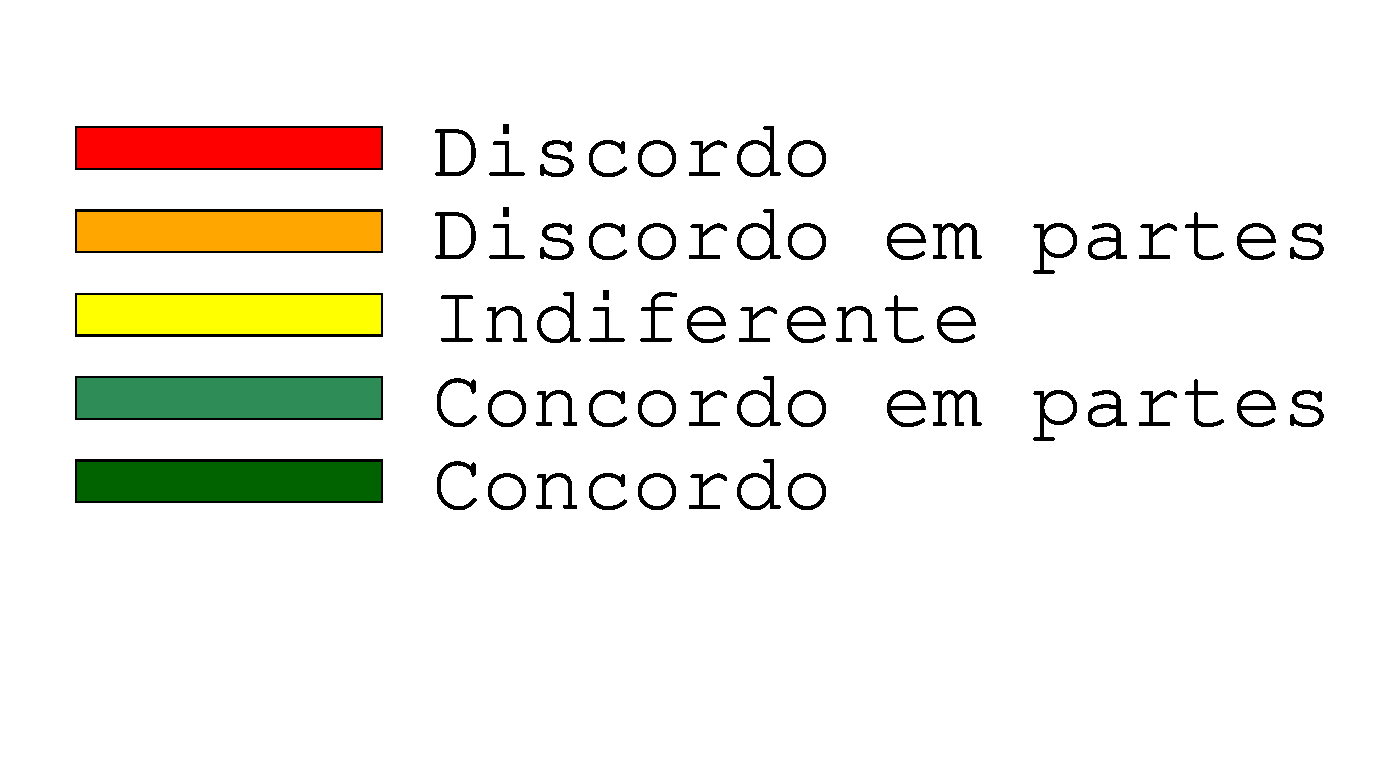
\includegraphics[scale=0.3,trim={0 4cm 0 1.5cm},clip]{figura-ref-graficos.eps}
\caption{Legenda para os gráficos em escala Likert} 
\label{figura-ref-graficos}
\end{figure}

\begin{table}[h]
\caption{Referências para os gráficos de percepção dos estudantes \textit{concluintes} sobre a disciplina}
\label{tabela-ref-graficos2}
\begin{tabular}{c|p{14.6cm}}
Legenda & Afirmativa respondida pelo participante \\
\hline
A & A metodologia da disciplina me agradou.\\
\hline
B & Gosto que a minha presença em sala faça parte da avaliação.\\
\hline
C & Gosto de ser avaliado pela participação durante as aulas.\\
\hline
D & Gosto de ter várias avaliações.\\
\hline
E & Gosto de avaliações em equipe.\\
\hline
F & Acredito que os tutores me motivaram suficientemente.\\
\hline
G & Consigo conciliar a disciplina com o trabalho profissional.\\
\hline
H & Eu entendi a metodologia PBL.\\
\hline
I & Falar em público é um grande problema para mim.\\
\hline
J & Eu gostaria de experimentar outras abordagens de ensino durante o meu curso além das aulas tradicionais.\\
\hline
K & A metodologia da disciplina me ajudou nas avaliações escritas (provas).\\
\hline
L & A metodologia da disciplina me ajudou a entender melhor a maioria dos conceitos estudados na disciplina.\\
\hline
M & A carga horária entre sessões tutorias e aulas expositivas foi suficientemente balanceada.\\
\hline
N & Tenho interesse em cursar outras disciplinas que possam utilizar esta abordagem.\\
\end{tabular}
\end{table}

\begin{table}[h]
\caption{Referências para os gráficos de percepção estudantes \textit{concluintes} sobre a disciplina}
\label{tabela-ref-graficos3}
\begin{tabular}{c|p{14.6cm}}
Legenda & Afirmativa respondida pelo participante \\
\hline
A & Desisti da disciplina porque a metodologia não me agradou.\\
\hline
B & Desisti da disciplina porque não gosto que a minha presença em sala faça parte da avaliação.\\
\hline
C & Desisti da disciplina porque não gosto de ser avaliado pela participação durante as aulas.\\
\hline
D & Desisti da disciplina porque não gosto de ter várias avaliações.\\
\hline
E & Desisti da disciplina porque não gosto de avaliações em equipe.\\
\hline
F & Desisti da disciplina porque acredito que os tutores não me motivaram suficientemente.\\
\hline
G & Desisti da disciplina porque não consigo conciliar a disciplina com o trabalho profissional.\\
\hline
G1 & Desisti da disciplina porque tive questões pessoais (exceto trabalho).\\
\hline
H & Eu entendi a metodologia PBL.\\
\hline
I & Falar em público é um grande problema para mim.\\
\hline
J & Eu gostaria de experimentar outras abordagens de ensino durante o meu curso além das aulas tradicionais.\\
\hline
N & Tenho interesse em cursar em breve a disciplina com esta abordagem.\\
\hline
M & Eu gostaria de experimentar a metodologia PBL, mas com mais carga horária de aulas expositivas.\\
\end{tabular}
\end{table}


Para cada um dos problemas foram construídos dois gráficos de resultados.
No primeiro gráfico são exibidos resultados para as respostas
dos participantes para questões afirmativas de percepção e
no segundo gráfico são exibidos os resultados para as notas atribuídas
ao problema pelo participante em uma avaliação geral.

Nos gráficos que seguem sobre as percepções dos participantes para os
problemas, a disposição nas barras
foi construída para facilitar a leitura por nível de favorabilidade.
No caso de analisar os resultados em uma perspectiva mais conservadora
para a favorabilidade, é possível considerar que apenas a concordância
integral, isto é, o participante respondeu ``concordo'' para
a afirmação como favorável.
A consideração de concordância em parte como favorável,
isto é, também considerar favorável que
o participante respondeu ``concordo em partes'' para a afirmação,
apresenta um resultado menos conservador em relação ao caso anterior.
E assim por diante, com a consideração da resposta `indiferente'', que
representará o caso de favorabilidade onde não há discordância de alguma forma,
etc.

Ao longo da discussão, ao mencionar textualmente uma afirmativa de
algum dos formulários, foi incluído entre parênteses a qual barra o texto
está se referindo, por exemplo, ``gosto da metologia PBL (X)''.

Nos gráficos para os resultados das notas atribuídas
ao problema pelo participante em uma avaliação geral,
existem duas projeções, sendo uma projeção de barras com
a leitura em $y_1$ à esquerda e uma projeção em curva
em $y_2$ à direita.
Ambas as projeções utilizam $x$ na parte de baixo para as notas
inteiras atribuídas de $0$ a $10$.
Em $y_1$ a leitura tem o significado de quantas respostas, valor absoluto,
que foram atribuídas para uma determinada nota, ou seja,
o tamanho da barra.
No caso de $y_2$ o significado é do percentil igual ou superior
(não inferior) a um determinado valor, isto é,
qual a porcentagem da distribuição das barras que é igual ou superior
a uma determinada nota.

Para as conclusões apresentadas neste trabalho sobre percepção foi
considerada que uma afirmação obteve resultado positivo
se obteve $70\%$ de favorabilidade,
sendo favoráveis as percepções com algum nível de concordância,
isto é, o participante respondeu ``concordo''
ou ``concordo parcialmente''.

Nas seções a seguir que detalham os resultados, serão discutidos apenas os
pontos principais observados, positivos e negativos, em torno da
favorabilidade para o resultado positivo dentro dos critérios
definidos no parágrafo anterior.
A discordância integral nas afirmativas será destacada para que
os possíveis pontos de melhoria estejam mais explicitados em meio
aos resultados positivos.

\section{Semestre 2016.1}
\label{sec-sem-2016}
\resultadoTurma{2016.1}{26}{9}{6}{57,7}{11}{8}{3}

\subsection{Problema 1 -- \ProblemaA}
\perfilProblema{\ProblemaA}{1}{2016.1}{14}
\perfilParticipante{27,9}{20}{51}{35,7}{71,4}{entre o terceiro e o quinto semestre}{}
\figuraPercepcaoParticipante{s1p1}{1}{2016.1}

É possível destacar que para todas as questões a favorabilidade
foi superior aos $70\%$. A favorabilidade foi superior aos $90\%$
para 12 afirmações apresentadas.
Apenas 6 afirmações receberam ao menos uma discordância integral.

A afirmação sobre ideias alternativas no caminho do problema (B)
foi a que teve a maior percepção de concordância por partes dos
participantes.
Entendemos que este resultado é explicado pelo problema
ter apresentado os conceitos de músicas, de forma que
os participantes precisaram realizar relacionamentos entre
os conceitos deste tema com os conceitos de linguagens
formais, e que os participantes perceberam que a depender do
nível de abstração poderá existir um caminho diferente.


A necessidade de recorrer aos materiais de apoio (D),
existência de informações suficientes no texto (K) e
sobre o participante gostar da metodologia baseada
em problemas (X) foram as afirmações com
as menores favorabilidades.
Embora possa parecer existir alguma contradição
sobre os resultados das duas primeiras, vale
ressaltar que os dados referente
a contribuição da sessão tutorial (Q) obtiveram
alta favorabilidade.

\figuraPercepcaoParticipanteNotas{s1p1}{1}{2016.1}{80}{5,00}{7,29}{quase}

\subsection{Problema 2 -- \ProblemaB}
\perfilProblema{\ProblemaB}{2}{2016.1}{12}
\perfilParticipante{28,5}{20}{51}{25,0}{75,0}{entre o terceiro e o quinto semestre}{}
\figuraPercepcaoParticipante{s1p2}{2}{2016.1}

Para 5 afirmações, na percepção dos estudantes, a favorabilidade foi integral.
Em 15 afirmações a favorabilidade superou os $90\%$.
Em apenas uma das afirmações a favorabilidade ficou pouco abaixo dos $70\%$, onde
$66,7\%$ dos participante acreditam que o problema estimulou
o trabalho em grupo (M).
Apenas 5 afirmações receberam ao menos uma discordância integral.

A contribuição dos tutores para a evolução do problema (U) foi a
afirmação melhor avaliada pelos participantes, assim como as demais
afirmações referentes aos tutores (W) e (V) também foram bem avaliadas,
indicando que os participantes aprovaram a participação
dos tutores na condução deste problema.

Para a construção do produto deste problema, os participantes
precisaram se reunir em equipe além das sessões tutoriais, desta forma,
acreditamos que as dificuldades referentes a se reunir fora das sessões tutorias
para trabalhar em grupo (M) estão também representados neste resultado.
Também observamos uma justificativa para este resultado ao analisar a favorabilidade para
a afirmação referente a percepção dos participantes com relação a quantidade
apropriada de estudantes em cada grupo tutorial (S).

\figuraPercepcaoParticipanteNotas{s1p2}{2}{2016.1}{70}{6,00}{7,17}{mais de}

\subsection{Problema 3 -- \ProblemaC}
\perfilProblema{\ProblemaC}{3}{2016.1}{8}
\perfilParticipante{31,4}{20}{51}{28,6}{85,7}{até o quinto semestre}{ para cada três participantes}
\figuraPercepcaoParticipante{s1p3}{3}{2016.1}

Para 7 afirmações, na percepção dos estudantes, a favorabilidade foi integral.
Em três afirmações a favorabilidade ficou abaixo dos $70\%$, mas apenas 2
afirmações receberam ao menos uma discordância integral.

A contribuição das sessões tutorias para o processo
de resolução do problema (Q) obteve a melhor avaliação pelos
participantes.
Entendemos que essa afirmação é bem avaliada sempre que
os participantes conseguem perceber uma informação de
grande relevância para a solução durante a sessão
tutorial, neste caso, a ideia de como manipular a pilha
de forma a manter a proporção exigida pelo problema
surgiu durante uma sessão tutorial.

No que diz respeito a quantidade de pessoas em
cada grupo tutorial (S) ser a afirmação a obter a pior
avaliação a justificativa pode ser obtida quando
é observada em conjunto com a afirmação referente ao
trabalho em equipe (M) que também esteve entre
as piores avaliações para este problema, neste caso,
ambos resultados são explicados pela quantidade de
participantes nas sessões tutoriais.

\figuraPercepcaoParticipanteNotas{s1p3}{3}{2016.1}{90}{6,00}{7,50}{quase}

\subsection{Problema 4 -- \ProblemaD}
\perfilProblema{\ProblemaD}{4}{2016.1}{8}
\perfilParticipante{31,5}{20}{51}{25,0}{87,5}{até o quinto semestre}{}
\figuraPercepcaoParticipante{s1p4}{4}{2016.1}

Para 12 afirmações, na percepção dos estudantes, a favorabilidade foi integral.
Em todas as afirmações a favorabilidade ficou acima dos $70\%$.
Em 4 afirmações foi recebida ao menos uma discordância integral.

A máquina de Turing foi o principal objetivo de aprendizagem para o Problema 4
aplicado no semestre 2016.1, sendo que para os participantes a afirmação
melhor avaliada diz respeito a utilidade dos conhecimentos aprendidos para 
o profissional da área de Computação (I).
Este problema foi muito bem avaliado pelos participantes para todas
as afirmações, mas cabe destacar os resultados para as afirmações que
dizem respeito a necessidade de aprender novos conhecimentos (G) e
motivação dos participantes para resolver o problema (E).

\figuraPercepcaoParticipanteNotas{s1p4}{4}{2016.1}{90}{5,00}{7,50}{quase}

\subsection{Problema 5 -- \ProblemaE}
\perfilProblema{\ProblemaE}{5}{2016.1}{7}
\perfilParticipante{32,3}{20}{51}{28,6}{71,4}{até o quinto semestre}{}
\figuraPercepcaoParticipante{s1p5}{5}{2016.1}

Para 6 afirmações, na percepção dos estudantes, a favorabilidade foi integral.
Em apenas duas afirmações a favorabilidade ficou abaixo dos $70\%$.
Em 9 afirmações foi recebida ao menos uma discordância integral, desta forma,
indicando vários pontos de atenção para a abordagem deste problema
em outras situações.

Este também foi um problema em que os participantes se reuniram em grupo para
construir uma solução, assim, como no Problema 2 no semestre 2016.1, a
afirmação pior avaliada também foi referente ao trabalho em equipe (M) que
indicamos que o resultado também inclui as dificuldades em se reunir além
das sessões tutoriais.

Ideias alternativas (B), utilização de referências bibliográficas (C),
recorrer a materiais não indicados nas referências (D), motivação
para resolver o problema (E), o tempo para resolução (L), a quantidade de
pessoas no grupo da sessão tutorial (S), utilidade do problema para o
processo de ensino e aprendizagem (T), \textit{feedback} dos
tutores (W), além da afirmação sobre o trabalho em equipe (M)
mencionado no parágrafo anterior, foram as afirmações com ao menos
uma discondância integral.
O mais possível é que este resultados sejam justificados pela sobrecarga
adicional que os estudantes possuem no fim do semestre, momento em que
este problema foi aplicado.
Ainda assim, não se deve desconsiderar que estes são pontos
de atenção claros, mas que mesmo em outras metodologias, com pesquisa
semelhante, os resultados da sobrecarga estariam também explicitados.

\figuraPercepcaoParticipanteNotasA{s1p5}{5}{2016.1}{70}{}{7,00}{pouco mais de}

\subsection{Percepção dos concluintes}

\subsection{Percepção dos desistentes}

\section{Semestre 2017.1}
\label{sec-sem-2017}
\resultadoTurma{2016.1}{50}{x}{y}{z}{a}{14}{b}


\subsection{Problema 1 -- \ProblemaG}
\label{sec-2017-p1}
\perfilProblema{\ProblemaG}{1}{2017.1}{12}
\perfilParticipante{26,1}{19}{44}{18,2}{72,7}
{até o terceiro semestre}{ para cada seis participantes}
\figuraPercepcaoParticipante{s2p1}{1}{2017.1}

Para 7 afirmações apresentadas a favorabilidade ficou um pouco abaixo dos $70\%$, mas
para 10 afirmações foi superior aos $90\%$.
Em 11 afirmações foi recebida ao menos uma discordância integral.

Neste problema com o objetivo de aprendizagem foi Linguagens
Formais, sendo consenso de percepção dos participantes que
este problema apresenta um conhecimento útil para um profissional
da área de Computação (I).

É possível destacar o excelente resultado para a afirmação que diz respeito a
utilidade do problema no processo de ensino e aprendizagem (T).
A explicação para este resultado está no fato de que os estudantes
conseguiram realizar bem as correlações entre os conceitos
do código Morse, apresentado no problema, com os conceitos de
linguagens formais, que são os objetivos de aprendizagem para
este problema.

Em uma análise mais detalhada dos dados foi possível
detectar que a discordância integral está concentrada
em 3 participantes, onde apenas um destes apresentou
5 discordâncias integrais.
Estes números além de indicar pontos possíveis de
priorização, também podem indicar a necessidade
de um nivelamento maior dos estudantes para a aplicação
da metodologia.

\figuraPercepcaoParticipanteNotas{s2p1}{1}{2017.1}{90}{5,00}{8,25}{quase}

\subsection{Problema 2 -- \ProblemaB}
\perfilProblema{\ProblemaB}{2}{2017.1}{13}
\perfilParticipanteA{24,3}{19}{38}{8,3}{63,6}
{até o terceiro semestre}{ quatro para cada dez}
\figuraPercepcaoParticipante{s2p2}{2}{2017.1}

A favorabilidade ficou um pouco abaixo dos $70\%$ em 6 afirmações apresentadas,
sendo superior aos $80\%$ em 12 afirmações.
Em 14 afirmações foi recebida ao menos uma discordância integral.

Neste problema o objetivo de aprendizagem principal foi
Autômatos Finitos, sendo consenso de percepção dos participantes que
este problema apresenta um conhecimento útil para um profissional
da área de Computação (I) e que é necessário aprender novos
conhecimentos (G).

Apenas um dos participantes respondeu com discordância integral para
8 afirmações, assim, também se faz necessário considerar a
necessidade de nivelamento do grupo, como mencionado
na Seção~\ref{sec-2017-p1}.

Apesar de obter favorabilidade muito próxima aos $70\%$, a afirmação
sobre o participante gostar da metodologia PBL (X) teve como
destaque negativo receber a maior discondância integral nessa
replicação.

\figuraPercepcaoParticipanteNotas{s2p2}{2}{2017.1}{60}{5,00}{7,31}{pouco mais de}

\subsection{Problema 3 -- \ProblemaC}
\perfilProblema{\ProblemaC}{3}{2017.1}{11}
\perfilParticipanteA{25,1}{19}{38}{0}{63,6}
{até o terceiro semestre}{ quatro para cada dez}
\figuraPercepcaoParticipante{s2p3}{3}{2017.1}

A favorabilidade ficou um pouco abaixo dos $70\%$ em apenas uma afirmação,
sendo superior aos $80\%$ para 21 destas afirmações.
Em apenas 2 afirmações foi recebida ao menos uma discordância integral.

Para este caso a percepção dos participantes
sobre a relevância das sessões tutorias no processo
de resolução do problema (Q), assim como no semestre
anterior, obteve favorabilidade integral, com o destaque de
que para este semestre todas as respostas recebidas foram de
total concordância.

A afirmativa pior avaliada diz respeito a percepção dos participantes
sobre o \textit{feedback} dos tutores a cada sessão tutorial (W).
Para este caso, apesar do resultado ainda ser alto, ficou como
um ponto de atenção aos tutores.

A Figura~\ref{aval-s2p3} apresenta o gráfico da
avaliação do participantes para o Problema 3 aplicado no semestre 2017.1.

\begin{figure}[!htb]
\centering
\includegraphics[scale=0.18]{notas-s2p3.eps}
\caption{Avaliação dos participantes do semestre 2017.1 para o Problema 3}
\label{aval-s2p3}
\end{figure}

Assim como no semestre anterior, este problema foi muito bem avaliado
pelos participantes, assim, todas as notas atribuídas foram maiores
ou iguais $7,00$ e uma média de $8,18$.

Entre os problemas que foram replicados em ambos os semestres, este
notadamente é o que apresentou as melhores avaliações pelos participantes
em todos os critérios, evidenciando o potencial da metodologia em uma
disciplina teórica com a utilização de um problema do ``mundo real''.

\subsection{Problema 4 -- \ProblemaD}
\perfilProblema{\ProblemaD}{4}{2017.1}{10}
\perfilParticipanteB{25,7}{19}{38}{11,1}{88,9}
{até o terceiro semestre}{igual}
\figuraPercepcaoParticipante{s2p4}{4}{2017.1}

Para todas as afirmativas a percepção dos participantes obteve favorabilidade
superior aos $70\%$. Em 5 afirmações foi recebida ao menos uma discordância
integral.

O destaque positivo para este problema foi a favorabilidade em relação
a necessidade de recorrer a materiais fora da bibliográfia básica (D).
Este é uma característica de estudo muito relevante no desenvolvimento
do estudante que passa a ver a necessidade de explorar fontes diversas
de informação para construir o seu conhecimento.

Como ponto de atenção, apesar de a favorabilidade ser igual aos $70\%$ para
a percepção do participante sobre a adequação do tempo disponível para desenvolver
a solução (L), houve uma quantidade relevante de discordância integral para esta afirmativa.

Este foi outro problema que foi bem avaliado em todos os critérios em ambos
os semestres.
\figuraPercepcaoParticipanteNotas{s2p4}{4}{2017.1}{80}{6,00}{7,31}{quase}

\subsection{Problema 5 -- \ProblemaE}
\perfilProblema{\ProblemaE}{5}{2017.1}{7}
\perfilParticipanteB{27,0}{20}{38}{20,0}{100,0}
{até o terceiro semestre}{semelhante}
\figuraPercepcaoParticipante{s2p5}{5}{2017.1}

Em 3 afirmações a favorabilidade ficou abaixo dos $70\%$ e 5 afirmações
receberam ao menos uma discordância integral.

Em contraste com o resultado que o mesmo problema teve com
os participantes do semestre 2016.1, onde foi a afirmação com a
pior favorabilidade, para os participantes neste semestre de
2017.1, a percepção de que o problema estimula o
trabalho em grupo (M) foi a afirmação melhor avaliada
para o Problema 5.
A diferença de resultado é justificada ao observar
a percepção dos participantes com relação a quantidade
apropriada de estudantes em cada grupo tutorial (S).

A afirmação com a menor favorabilidade diz respeito
a percepção de cumprimento dos objetivos de aprendizagem
pelo participante (F).
Neste ponto cabe destacar que ao apresentar um resultado
negativo para esta afirmação, uma vez que com outros
problemas dentro do mesmo grupo tiveram favorabilidade
melhores, se pode questionar o problema e não
a metodologia.
Também não se pode deixar de considerar o nível de abstração
mais elevado para o entendimento dos conceitos deste
problema em relação aos demais.

\figuraPercepcaoParticipanteNotas{s2p5}{5}{2017.1}{70}{5,00}{7,43}{pouco mais de}

\subsection{Percepção dos concluintes}
\figuraPercepcaoParticipanteDisciplina{concluintes-2017}{concluintes}{2017.1}

\subsection{Percepção dos desistentes}
\figuraPercepcaoParticipanteDisciplina{desistentes-2017}{desistentes}{2017.1}


\subsection{Percepção dos concluintes}
\QtdParticipantes{2016.1}{11}{1}{6}
\perfilParticipante{28,8}{20}{49}{50,0}{83,3}{até o quarto semestre}{}
\figuraPercepcaoParticipanteDisciplina{concluintes-2016}{concluintes}{2016.1}
\AprovacaoMetodologia{83,3}{concluintes}

\QtdParticipantes{2017.1}{x}{1}{12}
\perfilParticipanteB{22,75}{20}{28}{16,7}{58,3}{até o terceiro semestre}{semelhante}
\figuraPercepcaoParticipanteDisciplina{concluintes-2017}{concluintes}{2017.1}
\AprovacaoMetodologia{100,0}{concluintes}

\subsection{Percepção dos desistentes}
\QtdParticipantes{2016.1}{15}{0}{3}
\perfilParticipanteC{24,0}{23}{25}{66,7}{100,0}{até o sétimo semestre}{}
\figuraPercepcaoParticipanteDisciplina{desistentes-2016}{desistentes}{2016.1}
\AprovacaoDisciplina{0,0}{desistentes}{aprovação da metodologia para a}%
{a metodologia}{CA}

\QtdParticipantes{2017.1}{x}{0}{1}
\perfilParticipanteD{masculino}{23}{primeiro}{}{}
\figuraPercepcaoParticipanteDisciplina{desistentes-2017}{desistentes}{2017.1}
\AprovacaoDisciplina{0,0}{desistentes}{aprovação da metodologia para a}%
{a metodologia}{CA}


\section{Discussão}
\label{sec-avaliacao-hipoteses}
Para responder as hipóteses as quais este estudo se propõe, utilizamos
os resultados apresentados neste capítulo.
Inicialmente discutimos os resultados para as hipóteses
específicas e depois os resultados para as hispóteses gerais.

Para a avaliação das hipóteses deste estudo, uma vez que a
metologia utilizada exige que alguns critérios sejam
arbitrados, preferimos ser bastante conservadores
na definição dos parâmetros arbitrados.
No caso de uma hipótese como apenas uma afirmação, consideramos
a validade da hipótese se a afirmação recebe
resultado positivo dentro dos critérios mencionados na
Seção~\ref{sec-ref-graficos}, ou seja, $70\%$ de favorabilidade,
sendo favoráveis as respostas de concordância.
No caso de mais de uma afirmativa, consideramos a validade
da hipótese em caso de resultado positivo para todas
as afirmativas, dentro dos mesmos critérios.

Destacamos que a avaliação das hipóteses foi realizada para
cada replicação de problema, ou seja, é possível concluir pela
validade da hipótese em um problema, enquanto não é possível
em outro problema.

% HE1
\AvaliacaoHipotese{\heatexto}{he1ref}{he}{``\LikertPQ'' (Q)}{}{}{}{}{}

\AprovacaoHipotese{}{}{todas}{0}{}
\HipoteseFavorabilidadeDestaque{}{\ProblemaC}{2017.1}{100,0}{}{}
\HipoteseFavorabilidadeDestaqueContinuidade{2016.1}{100,0}{}
\HipoteseFavorabilidadeDestaqueDiferencas{2016.1}{25,0}{2017.1}{100,0}
\HipoteseFavorabilidadeDestaqueOutra{}{\ProblemaD}{2016.1}{100}{}
\HipoteseFavorabilidadeDestaqueContinuidade{2017.1}{90,0}{}
\AprovacaoHipoteseResultado{}{}{}{}{}{}{}{}{}

% HE2
\AvaliacaoHipotese{\hebtexto}{he2ref}{he}{``\LikertPM'' (M)}{}{}{}{}{}

\AprovacaoHipotese{}{não}{3}{0}{}
\AprovacaoHipoteseResultado{não}{\ProblemaB}{\ProblemaC}{\ProblemaE}{2016.1}{}{}{}{}
Em nosso trabalho \cite{gavaza2017}, que utilizamos apenas dados do
semestre 2016.1, apesar de não termos definidos parâmetros
de avaliação, percebemos que a percepção dos estudantes com relação
a motivação para o trabalho em equipe também não recebeu as melhores
avaliações.
No semestre 2016.1, como descrito na Seção ~\ref{sec-exp-2016}, foi utilizado
apenas um quadro branco, assim foi formado apenas um grupo com todos
os estudantes.
Para o semestre 2017.1, como descrito na Seção ~\ref{sec-exp-2017}, foram
utilizados quadros adicionais e foram formados grupos menores,
de até dez participantes cada.
\AprovacaoHipotese{}{}{todas}{0}{2017.1}
\HipoteseFavorabilidadeDestaque{}{\ProblemaE}{}{100,0}{85,7}{}
% escrever sobre a redução no grupo tutorial e qual a conclusão

% HE3
\AvaliacaoHipotese{\hectexto}{he3ref}{he}{``\LikertPT'' (T)}{}{}{}{}{}

\AprovacaoHipotese{}{}{todas}{0}{}
\HipoteseFavorabilidadeDestaque{}{\ProblemaC}{2016.1}{100,0}{50,0}{\ProblemaD}
\HipoteseFavorabilidadeDestaqueContinuidade{2017.1}{90,9}{80,0}
\HipoteseFavorabilidadeDestaqueOutra{}{\ProblemaG}{2017.1}{91,7}{91,7}
\ProblemaSemReplica{2016.1}{}
\AprovacaoHipoteseResultado{}{}{}{}{}{}{}{}{}

% HE4
\AvaliacaoHipotese{\hedtexto}{he4ref}{he}{``\LikertPC'' (C)}{``\LikertPD'' (D)}
{``\LikertPG'' (G)}{``\LikertPK'' (K)}{``\LikertPO'' (O)}{``\LikertPP'' (P)}

\HipoteseNaoAtende{\ProblemaG}{2017.1}{(C)}{(D)}{(O)}{}{}{}{}
\ProblemaSemReplica{2016.1}{\ProblemaG}
\HipoteseNaoAtende{\ProblemaB}{2017.1}{(C)}{(D)}{(P)}{}{}{}{}
\HipoteseAtende{\ProblemaB}{2016.1}{p}
\AprovacaoHipotese{}{não}{2}{1}{}
\AprovacaoHipoteseResultado{não}{\ProblemaG}{\ProblemaB}{}{2017.1}{}{}{}{}

% HE5
\AvaliacaoHipotese{\heetexto}{he5ref}{he}{``\LikertPU'' (U)}{``\LikertPV'' (V)}
{``\LikertPW'' (W)}{}{}{}

\HipoteseNaoAtende{\ProblemaG}{2017.1}{(W)}{}{}{}{}{}{}
\HipoteseAtende{\ProblemaG}{2016.1}{p}
\HipoteseNaoAtende{\ProblemaB}{2017.1}{(W)}{}{}{}{}{}{}
\HipoteseAtende{\ProblemaB}{2016.1}{p}
\HipoteseNaoAtende{\ProblemaC}{2017.1}{(W)}{}{}{}{}{}{}
\HipoteseAtende{\ProblemaC}{2016.1}{p}
\HipoteseNaoAtende{\ProblemaE}{2017.1}{(W)}{}{}{}{}{}{}
\HipoteseAtende{\ProblemaE}{2016.1}{p}
A favorabilidade não foi atingida em 4 das 5 replicações no
semestre 2017.1.

% HE6
\AvaliacaoHipotese{\heftexto}{he6ref}{he}{``\LikertPI'' (I)}{}{}{}{}{}

\AprovacaoHipotese{}{}{todas}{0}{}
\HipoteseFavorabilidadeDestaque{}{\ProblemaC}{2017.1}{100,0}{90,9}{}
\HipoteseFavorabilidadeDestaqueContinuidade{2016.1}{75,0}{}
\MaisDestaque{4}{5}{2017.1}{85,8}{\ProblemaE}
\AprovacaoHipoteseResultado{}{}{}{}{}{}{}{}{}

% HE7
\AvaliacaoHipotese{\hegtexto}{he7ref}{he}{``\LikertPA'' (A)}{``\LikertPB'' (B)}{}{}{}{}

\HipoteseNaoAtende{\ProblemaE}{2016.1}{(B)}{}{}{}{}{}{}
\HipoteseAtende{\ProblemaE}{2017.1}{p}
\HipoteseNaoAtende{\ProblemaG}{2017.1}{(B)}{}{}{}{}{}{}
\ProblemaSemReplica{2017.1}{\ProblemaG}
\AprovacaoHipoteseResultado{não}{\ProblemaE}{}{}{2016.1}{\ProblemaG}{}{}{2017.1}

% HG1
\AvaliacaoHipotese{\hgatexto}{hg1ref}{hg}{``\LikertPX'' (X)}{}{}{}{}{}

\AprovacaoHipotese{}{não}{3}{0}{}
\AprovacaoHipoteseResultado{não}{\ProblemaC}{}{}{2016.1}{\ProblemaB}{\ProblemaE}{}{2017.1}
\HipoteseFavorabilidadeDestaque{}{\ProblemaD}{2016.1}{87,5}{}{}
\HipoteseFavorabilidadeDestaqueContinuidade{2017.1}{70,0}{}

% HG2
\AvaliacaoHipotese{\hgbtexto}{hg2ref}{hg}{``\LikertPF'' (F)}{}{}{}{}{}

\AprovacaoHipotese{}{não}{1}{0}{}
\AprovacaoHipoteseResultado{não}{\ProblemaE}{}{}{2017.1}{}{}{}{}
\HipoteseFavorabilidadeDestaque{}{\ProblemaD}{2016.1}{100,0}{37,5}{}
\HipoteseFavorabilidadeDestaqueContinuidade{2017.1}{70,0}{}

% HG3
\AvaliacaoHipotese{\hgctexto}{hg3ref}{hg}{``\LikertPE'' (E)}{}{}{}{}{}

\AprovacaoHipotese{}{}{todas}{0}{}
\HipoteseFavorabilidadeDestaque{}{\ProblemaA}{2016.1}{92,9}{42,9}{}
\ProblemaSemReplica{2017.1}{\ProblemaA}
\HipoteseFavorabilidadeDestaqueOutra{}{\ProblemaG}{2017.1}{91,7}{25,0}
\ProblemaSemReplica{2016.1}{\ProblemaG}
\HipoteseFavorabilidadeDestaqueOutra{}{\ProblemaB}{2016.1}{91,7}{50,0}
\HipoteseFavorabilidadeDestaqueContinuidade{2017.1}{77,0}{}
\AprovacaoHipoteseResultado{}{}{}{}{}{}{}{}{}

\section{Considerações finais}
\label{sec-consideracoes-resultados}
% resumo básico
Neste capítulo foram apresentados os resultados do estudo no contexto de execução onde foi aplicada a
metologia PBL em dez replicações de problemas em duas turmas de estudantes e apresentada a discussão
das hipóteses deste estudo.

% dificuldade em obter respostas
Uma das principais dificuldades deste trabalho foi adesão
por partes dos estudantes em responder os formulários,
como pode ser observado calculando a razão entre
a quantidade de respostas obtidas no formulário de
replicação dos problemas e a quantidade de estudantes
na turma.
A adesão ficou entre $14\%$ e $46\%$, na
quinta replicação do semestre 2017.1 e na primeira
replicação do semestre 2016.1, respectivamente.
Neste cálculo foi considerado a quantidade de estudantes
que iniciaram no semestre, portanto, não foi considerado os
estudantes que eventualmente já haviam desistido
da disciplina.
Acreditamos que a adesão poderia ser melhor se existisse
institucionalmente, desde o ingresso dos estudantes,
ampla divulgação aos estudantes da importância das pesquisas
científicas na construção do conhecimento e que os resultados,
como se propõe este estudo, podem trazer novas oportunidades
para o ensino.

Como foi destacado pelos revisores do nosso trabalho \cite{gavaza2017},
outra questão que devemos observar é que, na metodologia de pesquisa
que adotamos, pode existir uma maior possibilidade
de adesão em responder as pesquisas por partes
dos estudantes ``mais interessados'', portanto, poderiam
estes apresentar uma maior tendência a aceitação.
Embora entendamos a possibilidade desta relação, obervamos que
neste estudo também existiram respostas em sentido
contrário, explicitamos um exemplo na discussão da
replicação do problema ``\ProblemaG'', no semestre 2017.1,
na Seção~\ref{sec-2017-p1}, onde exibimos a existência
de participantes que apresentaram discordância intregal
para afirmativas.

% não compartivo
O experimental deste estudo não foi construído como comparativo
entre metodologias, portanto, não há indicação, nesse
contexto, para a utilização da metologia deste estudo
em substituição a alguma outra metodologia, inclusive uma
metodologia tradicional.

Além de uma infraestrura adicional, para um estudo conter
aplicações de abordagens distintas em mais de uma turma,
se faz necessário construir ou investigar critérios de
comparabilidade, que também não foi o propósito deste estudo,
assim, a maioria das afirmativas utilizadas neste estudo
estão focadas em especificidades da metodologia PBL.

% resultados negativos

% resultados positivos

\xchapter{Conclusões}{} %sem preambulo
% É recomendável utilizar `\acresetall' no início de cada capítulo para reiníciar o contator de referências às siglas.
\acresetall
\section{Trabalhos futuros}

% ...
% \include{capituloN}
%

%% Parte pos-textual
\backmatter

% Bibliografia
% É aconselhável utilizar o BibTeX a partir de um arquivo, digamos "biblio.bib".
% Para ajuda na criação do arquivo .bib e utilização do BibTeX, recorra ao
% BibTeXpress em www.cin.ufpe.br/~paguso/bibtexpress
\bibliographystyle{abntex2-alf}
\bibliography{biblio}

% Apendices
% Comente se naoo houver apendices
 \appendix

%\xchapter{Exemplo de Ap^endice}{} %sem preambulo
%\lipsum
% Eh aconselhavel criar cada apendice em um arquivo separado, digamos
% "apendice1.tex", "apendice.tex", ... "apendiceM.tex" e depois
% inclui--los com:
\xchapter{Termo de consentimento livre e esclarecido}{}
\acresetall
\label{termo-ciencia}
Você está sendo convidado(a) a participar, como voluntário(a), do estudo/pesquisa
intitulado(a) aplicação da metodologia PBL no ensino da disciplina MATC94 da UFBA,
conduzida por Luiz Otávio Ramos Gavaza, sob orientação de Laís do Nascimento Salvador
e David Moises Barreto dos Santos.
Este estudo tem por objetivo avaliar a aderência da metodologia PBL para
a disciplina em questão.
Você foi selecionado(a) por ser aluno regularmente matriculado na disciplina em questão.
Sua participação não é obrigatória.
A qualquer momento, você poderá desistir de participar e retirar seu consentimento.
Sua recusa, desistência ou retirada de consentimento não acarretará prejuízo.
O principal risco ao qual você está submetido é o de não entendimento da metodologia
e que será mitigado com uma sessão de exemplo da metodologia.
A sua participação não trará quaisquer vantagens ou prejuízos de qualquer natureza
para você, isso incluí financeiro e notas na disciplina.
Sua participação nesta pesquisa consistirá em realizar as atividades propostas
em sala de aula, responder questionários disponíveis no espaço da disciplina
no Moodle UFBA e eventualmente participar de entrevistas realizadas em ambientes
da UFBA onde poderão ser registrados áudio, de vídeo ou imagem.
Os dados obtidos por meio desta pesquisa serão confidenciais e não serão
divulgados em nível individual, visando assegurar o sigilo de sua participação.
O pesquisador responsável se comprometeu a tornar públicos nos meios acadêmicos
e científicos os resultados obtidos de forma consolidada sem qualquer identificação
de indivíduos participantes.
Caso você concorde em participar desta pesquisa, você deverá realizar a
assinatura digital ou física deste termo.
Segue o email e telefone do pesquisador responsável, onde você poderá tirar
suas dúvidas sobre o projeto e sua participação nele, agora ou
a qualquer momento.
Contatos do pesquisador responsável: Luiz Otávio Ramos Gavaza, mestrando,
lgavaza@ufba.br e $<$telefone omitido$>$.

\xchapter{Formulário de percepção de participante sobre problema}{}
\acresetall
\label{form-problema}
\begin{enumerate}
\item{Idade}
\item{Sexo}
\begin{itemize}
	\item{Feminino}
	\item{Masculino}
\end{itemize}
\item{Ano/Semestre que iniciou o curso}
\AfirmacaoSimNao{Já trancou ou desistiu da disciplina antes?}
\AfirmacaoSimNao{Já trancou ou desistiu de outra
disciplina no curso alguma vez?}
\AfirmacaoLikert{\LikertPA{}}
\AfirmacaoLikert{\LikertPB{}}
\AfirmacaoLikert{\LikertPC{}}
\AfirmacaoLikert{\LikertPD{}}
\AfirmacaoLikert{\LikertPE{}}
\AfirmacaoLikert{\LikertPF{}}
\AfirmacaoLikert{\LikertPG{}}
\AfirmacaoLikert{\LikertPH{}}
\AfirmacaoLikert{\LikertPI{}}
\AfirmacaoLikert{\LikertPJ{}}
\AfirmacaoLikert{\LikertPK{}}
\AfirmacaoLikert{\LikertPL{}}
\AfirmacaoLikert{\LikertPM{}}
\AfirmacaoLikert{\LikertPN{}}
\AfirmacaoLikert{\LikertPO{}}
\AfirmacaoLikert{\LikertPP{}}
\AfirmacaoLikert{\LikertPQ{}}
\AfirmacaoLikert{\LikertPR{}}
\AfirmacaoLikert{\LikertPS{}}
\AfirmacaoLikert{\LikertPT{}}
\AfirmacaoLikert{\LikertPU{}}
\AfirmacaoLikert{\LikertPV{}}
\AfirmacaoLikert{\LikertPW{}}
\AfirmacaoLikert{\LikertPX{}}
\item{Fazendo uma avaliação geral do problema, que nota você
atribuiria a ele? Atribua uma nota de 0 a 10. (0 - 10)}
\item{Espaço para exposição livre sobre o problema:}
\item{Espaço para exposição livre sobre percepção do método PBL:}
\end{enumerate}

\xchapter{Formulário de percepção sobre a disciplina de participante concluinte}
\acresetall
\label{form-disciplina-concluinte}
\begin{enumerate}
\item{Idade}
\item{Sexo}
\begin{itemize}
	\item{Feminino}
	\item{Masculino}
\end{itemize}
\item{Ano/Semestre que iniciou o curso}
\AfirmacaoSimNao{Já trancou ou desistiu da disciplina antes?}
\AfirmacaoSimNao{Já trancou ou desistiu de outra
disciplina no curso alguma vez?}
\AfirmacaoLikert{\LikertCA{}}
\AfirmacaoLikert{\LikertCB{}}
\AfirmacaoLikert{\LikertCC{}}
\AfirmacaoLikert{\LikertCD{}}
\AfirmacaoLikert{\LikertCE{}}
\AfirmacaoLikert{\LikertCF{}}
\AfirmacaoLikert{\LikertCG{}}
\item{Qual você considera o maior motivador desta disciplina MATC94 neste semestre?}
\begin{itemize}
\item{A metodologia da disciplina.}
\item{A minha presença em sala fazer parte da avaliação.}
\item{Ser avaliado pela participação em todas as aulas.}
\item{Ter várias avaliações.}
\item{Os trabalhos em equipe.}
\item{A motivação pelos tutores.}
\item{Outra razão não listada (por favor, mencione no espaço aberto abaixo).}
\end{itemize}
\AfirmacaoLikert{\LikertCH{}}
\AfirmacaoLikert{\LikertCI{}}
\AfirmacaoLikert{\LikertCJ{}}
\AfirmacaoLikert{\LikertCK{}}
\AfirmacaoLikert{\LikertCL{}}
\AfirmacaoLikert{\LikertCM{}}
\AfirmacaoSimNao{Você participou da sessão tutorial de exemplo?}
\AfirmacaoLikert{\LikertCN{}}
\item{Fazendo uma avaliação geral do problema, que nota você
atribuiria a ele? Atribua uma nota de 0 a 10. (0 - 10)}
\item{Espaço para exposição livre sobre percepção do método PBL:}
\item{Espaço para exposição livre sobre a disciplina:}
\end{enumerate}

\xchapter{Formulário de percepção sobre a disciplina de participante desistente}
\acresetall
\label{form-disciplina-desistente}
\begin{enumerate}
\item{Idade}
\item{Sexo}
\begin{itemize}
	\item{Feminino}
	\item{Masculino}
\end{itemize}
\item{Ano/Semestre que iniciou o curso}
\AfirmacaoSimNao{Já trancou ou desistiu da disciplina antes?}
\AfirmacaoSimNao{Já trancou ou desistiu de outra
disciplina no curso alguma vez?}
\AfirmacaoLikert{\LikertDA{}}
\AfirmacaoLikert{\LikertDB{}}
\AfirmacaoLikert{\LikertDC{}}
\AfirmacaoLikert{\LikertDD{}}
\AfirmacaoLikert{\LikertDE{}}
\AfirmacaoLikert{\LikertDF{}}
\AfirmacaoLikert{\LikertDG{}}
\AfirmacaoLikert{\LikertDGa{}}
\item{Qual você considera o maior motivador para você desistir de
cursar a disciplina MATC94 neste semestre?}
\begin{itemize}
\item{A metodologia da disciplina não me agradou.}
\item{Não gosto que a minha presença em sala faça parte da avaliação.}
\item{Não gosto de ser avaliado pela participação em todas as aulas.}
\item{Não gosto de ter várias avaliações.}
\item{Não gosto de trabalhos em equipe.}
\item{Os tutores não me motivaram suficientemente.}
\item{Não consigo conciliar a disciplina com o trabalho profissional.}
\item{Tive questões pessoais (exceto trabalho).}
\item{Outra razão não listada (por favor, mencione no espaço aberto abaixo).}
\end{itemize}
\AfirmacaoLikert{\LikertDH{}}
\AfirmacaoLikert{\LikertDI{}}
\AfirmacaoLikert{\LikertDJ{}}
\AfirmacaoLikert{\LikertDO{}}
\AfirmacaoSimNao{Você participou da sessão tutorial de exemplo?}
\item{Em quantas sessões tutoriais você esteve presente?}
\begin{itemize}
\item{0}
\item{1}
\item{2}
\item{3}
\item{4}
\item{5 ou mais}
\end{itemize}
\AfirmacaoLikert{\LikertDOa{}}
\item{Fazendo uma avaliação geral do problema, que nota você
atribuiria a ele? Atribua uma nota de 0 a 10. (0 - 10)}
\item{Espaço para exposição livre sobre percepção do método PBL:}
\item{Espaço para exposição livre sobre a disciplina:}
\end{enumerate}

\newcommand{\tituloProblema}[2]{\textbf{\\#1. #2\\}}
\xchapter{Problemas}{}
\acresetall
\label{cap-problemas-textos}
\section{\ProblemaA}
\tituloProblema{1}{Problema}
Um certo colecionador de arte dispõe de partituras e gravações de
músicas, as quais ele precisa catalogar e processar mediante computador.
O colecionador em questão é muito exigente com o tratamento do seu material e
garante que para cada música na sua coleção, a partitura corresponde exatamente com
a gravação correspondente.

Algumas das partituras que o colecionador possui são para apenas um
instrumento.
Outras são para vários instrumentos.
Cada partitura para um instrumento pode ser vista como uma sequência de
símbolos musicais.
No caso das partituras para vários instrumentos, elas podem ser vistas
como sequências, mas de símbolos compostos: cada elemento da sequência é formado por um número finito
de símbolos musicais.
Cada música pode ter um número arbitrário de símbolos.

Veja a seguir exemplos de partituras.

Um instrumento:\\
\begin{abc}[name=um]
X:1
M:2/4
K:G
[L:1/4] G/A/ | B d | d B | c c |
\end{abc}

Note que cada nota pode ser vista de forma independente como um símbolo (escrito em um pentagrama). No exemplo a seguir, correspondente a uma partitura para três instrumentos, cada um deles possui uma representação similar à vista acima: Cada instrumento possui o seu próprio pentagrama e em cada um deles, os símbolos são superpostos em cada tempo.

Três instrumentos:\\
\begin{abc}[name=tres]
X: 1
M: 3/4
L: 1/4
V:1 name="Flauta" clef=treble
V:2 name="Baixo" clef=treble
V:3 name="Piano" clef=treble
K:Gm
%
[V:1] |: b d' b/g/ | ^f d a
[V:2] |: G B G | d ^f d 
[V:3] |: G/A/ b  B | d A c
\end{abc}

No caso das partituras para vários instrumentos, elas
também podem ser vistas como sequências, mas de símbolos
compostos: cada elemento da sequência é formado
por um número finito de símbolos musicais, sendo um
em cada instrumento.

Apesar de bastante exigente, este colecionador não entende muito bem sobre linguagens,
mas ele gostaria de ter um sistema automatizado que pudesse criar novas composições
a partir das que já possui.

O colecionador ficou sabendo que os alunos desta turma de Introdução as Linguagens Formais
e Teoria da Computação da UFBA estão estudando sobre linguagens formais, então decidiu pedir
ajuda para que eles idealizassem o sistema.

Ele disponibilizou toda a coleção e listou algumas restrições que o sistema
deve atender para que ele fique satisfeito.

\begin{enumerate}
\item O colecionador quer que ao menos duas músicas sejam utilizadas como base para gerar uma nova música,
onde apenas símbolos existentes nas músicas utilizadas como base podem ser utilizadas para uma nova composição;
\item O colecionador gostaria que o sistema fosse capaz de criar músicas para uma quantidade variada de instrumentos;
\item Em ao menos $10\%$ e no máximo $20\%$ das superposições dos símbolos, isto é, quando a nova composição for para mais de um instrumento,
o colecionador gostaria de ouvir a mesma nota em todos os instrumentos da nova composição;
\item O colecionador quer que pequenos trechos das músicas utilizadas como base estejam
presentes nas novas composições;
\item O colecionador quer ter certeza que as novas composições contemplam o máximo
de operações existentes em linguagens formais estudadas pelos alunos, então pediu para
que eles assim fizessem, além de incluir detalhadamente ao menos um exemplo de cada operação
no relatório.
\end{enumerate}

\tituloProblema{2}{Produto}
Uma nova coleção de músicas com no mínimo 10 composições geradas conforme as exigências do colecionador
para demonstrar que é capaz de desenvolver o sistema idealizado, bem como, um relatório no modelo de
artigos da SBC que descreva com o máximo de detalhes a idealização de funcionamento do sistema, onde deverá
constar quais as operações executadas pelo sistema para criação das músicas e incluir ao menos
um exemplo de cada uma das operações sob linguagens formais utilizadas pelo sistema idealizado.

\tituloProblema{3}{Cronograma}
4 sessões tutoriais e 1 aula expositiva.

\tituloProblema{4}{Recursos para aprendizagem}
RAMOS, M. V. M.; JOSÉ NETO, J.; VEGA, I. S. \textbf{Linguagens Formais: Teoria, Modelagem e Implementação}. Editora Bookman, 2009.\\

\noindent
MENEZES, Paulo Blauth. \textbf{Linguagens formais e autômatos}. 6. ed. Bookman, 2011.\\

\noindent
https://hudlac.wordpress.com/notacao-musical-abc\\

\noindent
http://abcnotation.com

\tituloProblema{$*$}{Referências}
Este problema é baseado nas notas de aula do professor Martin Musicante\footnote{\scriptsize{https://sigaa.ufrn.br/sigaa/public/docente/portal.jsf?siape=1221251}} do DIMAP - UFRN.

\newpage
\section{\ProblemaB}
\tituloProblema{1}{Problema}
A empresa \textit{Refrigerantes e Salgados S.A.} resolveu desenvolver novas soluções
para as suas máquinas de vender refrigerantes e salgados
baseadas em autômatos finitos.

A ideia surgiu quando um dos representantes de vendas da empresa estava conversando
com um grupo de alunos da disciplina de Teoria da Computação da UFBA.
Eles perceberam que os autômatos finitos e expressões regulares
atendem as necessidades das máquinas e que são
de simples configuração.

%O representante de vendas resolveu que iria fornecer alguns materiais aos alunos para
%que eles idealizassem as máquinas.

%Foi entregue aos alunos sensores capazes de identificar as moedas e notas brasileiras.
%Os alunos receberam também um sistema capaz de ser programado exatamente como um
%autômato finito

O representante de vendas falou aos alunos que soube que a equipe de tecnologia
da empresa utiliza uma ferramenta chamada de JFLAP\footnote{http://www.jflap.org}
para testar outras soluções que utilizam autômatos finitos.

As máquinas devem ser configuradas para vender no mínimo três produtos e
receber notas de R\$ 2,00 e R\$ 5,00.

O representante de vendas disse aos alunos que para ajudar na divulgação
das novas máquinas irá realizar uma promoção, onde as máquinas deverão
considerar aleatoriamente a possibilidade de dar um troco de R\$ 2,00
como prêmio para o caso de o valor inserido pelo cliente ser exatamente
o preço do produto selecionado.

O representante de vendas soube da equivalência entre autômatos finitos
e expressões regulares, logo solicitou que seja construída uma expressão
regular geral para representar à máquina.

\tituloProblema{2}{Produto}
Um arquivo com um autômato finito que contenha a máquina de vender
refrigerantes e salgados de forma que a equipe de tecnologia da
empresa \textit{Refrigerantes e Salgados S.A.} possa testar, ou seja, no JFLAP,
a expressão regular, bem como, um relatório no modelo de
artigos da SBC que descreva com o máximo de detalhes a idealização de funcionamento do
sistema da máquina de vender refrigerantes e salgados, onde deverá
constar quais as operações executadas pelo sistema para receber o pagamento pelo cliente e entregar o
produto escolhido e ao menos 2 exemplos de funcionamento, tanto com autômatos
como com expressões regulares.

\tituloProblema{3}{Cronograma}
2 sessões tutoriais e 1 aula expositiva.

\tituloProblema{4}{Recursos para aprendizagem}
RAMOS, M. V. M.; JOSÉ NETO, J.; VEGA, I. S. \textbf{Linguagens Formais: Teoria, Modelagem e Implementação}. Editora Bookman, 2009.\\

\noindent
MENEZES, Paulo Blauth. \textbf{Linguagens formais e autômatos}. 6. ed. Bookman, 2011.\\

\tituloProblema{$*$}{Referências}
Este problema é baseado nas notas de aula do professor Martin Musicante\footnote{\scriptsize{https://sigaa.ufrn.br/sigaa/public/docente/portal.jsf?siape=1221251}} do DIMAP - UFRN.

\newpage
\section{\ProblemaC}
\tituloProblema{1}{Problema}
Um dos problemas que afetam as rodovias brasileiras são os buracos.
Muitos são os motivos que podem causar este problema, sendo a alternância de chuva e sol
um dos motivos que pode acelerar o desgaste do asfaltamento e consequentemente gerar buracos.
Outro motivo é o tráfego intenso de veículos, em particular a frequência com que veículos
pesados empregam as estradas.

Na estrada de Aratu, em Salvador, alguns buracos foram identificados pelos
técnicos da Superintendência de Infraestrutura de Transportes da Bahia (SIT-BA).
Os técnicos desta Superintendência acreditam que
podem reduzir a pressão sobre o asfaltamento, desta forma, melhorar o
problema dos buracos, se conseguirem aplicar um controle de
tráfego.

A ideia é separar os veículos em categorias leve e pesado, onde os
veículos até $6$ (seis) toneladas são leves e acima deste peso são pesados.

Os técnicos informaram que a proporção atual de veículos que trafegam na
estrada durante um dia é de $3$ (três) veículos pesados
para cada $5$ (cinco) veículos leves.

O controle de tráfego a ser utilizado deverá, a cada dia, gradativamente,
reduzir a proporção de veículos pesados trafegando na estrada até que a média
ao final do dia seja no máximo $1$ (um) veículo pesado
para cada $5$ (cinco) veículos leves.

Você pode considerar que existe uma balança na entrada da estrada para realizar a pesagem
dos veículos.
Também pode considerar que há uma rota alternativa mais longa em que os veículos
só serão encaminhados por este caminho para atender as restrições
do controle de tráfego, uma vez que se deseja obter o máximo de vasão
possível na estrada principal obedecendo as restrições.

\tituloProblema{2}{Produto}
(i) Autômatos de Pilha necessários para utilização no controle de tráfego descrito;
(ii) um relatório no modelo de artigos da SBC que descreva com o máximo de detalhes a idealização de funcionamento deste
sistema de controle de tráfego;
e (iii) construir gramáticas livre de contexto equivalentes aos autômatos construídos na solução.
As dificuldades ou não possibilidade de construção de gramática para algum dos autômatos construídos
deverá constar no relatório mencionado no item (ii).

\tituloProblema{3}{Cronograma}
4 sessões tutoriais e 1 aula expositiva.

\tituloProblema{4}{Recursos para aprendizagem}

RAMOS, M. V. M.; JOSÉ NETO, J.; VEGA, I. S. \textbf{Linguagens Formais: Teoria, Modelagem e Implementação}. Editora Bookman, 2009.\\

\noindent
MENEZES, Paulo Blauth. \textbf{Linguagens formais e autômatos}. 6. ed. Bookman, 2011.\\

\newpage
\section{\ProblemaD}
\tituloProblema{1}{Problema}
Um dos problemas que afetam as rodovias brasileiras são os buracos.
Muitos são os motivos que podem causar este problema, sendo a alternância de chuva e sol
um dos motivos que pode acelerar o desgaste do asfaltamento e consequentemente gerar buracos.
Outro motivo é o tráfego intenso de veículos, em particular o peso com que veículos
pesados empregam nas estradas durante o pernoite.

Na estrada de Aratu, em Salvador, alguns buracos foram identificados pelos
técnicos da Superintendência de Infraestrutura de Transportes da Bahia.
Os técnicos desta Superintendência acreditam que
podem reduzir a pressão sobre o asfaltamento, desta forma, melhorar o
problema dos buracos, se conseguirem aplicar uma melhoria no controle de tráfego
da rodovia.

Os veículos são categorizados em: leves, pesados e muito pesados.
Veículos de até $6$ (seis) toneladas são leves;
acima de $6$ (seis) e abaixo de $10$ (dez) toneladas são pesados;
e de $10$ (dez) ou mais toneladas são muito pesados.

Já existem sensores nas entradas e nas saídas da estrada que permitem identificar a
categoria dos veículos que entram e saem da rodovia.

Os técnicos esperam uma solução que, a partir das informações dos
sensores, seja capaz de realizar a contagem de quantos veículos
de cada categoria passaram a noite estacionados na estrada (pernoite) e também apontar
a categoria que teve mais veículos no pernoite.

\tituloProblema{2}{Produto}
(i) Um arquivo com uma máquina de Turing que contenha a solução para o
problema; e (ii) um relatório no modelo de artigos da SBC que descreva com o máximo
de detalhes a idealização de funcionamento do sistema de controle de tráfego com a
melhoria de identificar quais as categorias que estão passando a noite na estrada.

\tituloProblema{3}{Cronograma}
2 sessões tutoriais e 2 aulas expositivas.

\tituloProblema{4}{Recursos para aprendizagem}

RAMOS, M. V. M.; JOSÉ NETO, J.; VEGA, I. S. \textbf{Linguagens Formais: Teoria, Modelagem e Implementação}. Editora Bookman, 2009.\\

\noindent
MENEZES, Paulo Blauth. \textbf{Linguagens formais e autômatos}. 6. ed. Bookman, 2011.\\

\noindent
HOPCROFT, John E.; ULLMAN, Jeffrey D.; MOTWANI, Rajeev. \textbf{Introdução à teoria de autômatos, linguagens e computação}. Editora Campus, 2002.\\

\noindent
SIPSER, Michael. \textbf{Introdução à teoria da computação}. Thomson Learning, 2007.

\newpage
\section{\ProblemaE}
\subsection{Problema}
Todos os compiladores da linguagem C tomam como entrada um código fonte de um
programa e produzem como saída um código executável.
Os compiladores podem ser bastante sofisticados. Por exemplo, eles
podem detectar erros de sintaxe, podem também indicar alguns erros de
semântica (como o uso de ``='' em uma situação que normalmente pede-se ``==''),
eles podem otimizar o código resultante em termos de tempo e/ou memória consumidos.

O quanto inteligente um compilador pode ser?
Por exemplo, ele poderia detectar que todos os valores de entrada negativos
levam o seguinte programa a entrar em um \textit{loop} infinito?

\lstinputlisting{apendice/problemas/problema5/codigo1.c}

Talvez compiladores não sejam assim tão sofisticados, mas será
que seriam capazes de responder uma questão geral, como:
\\ \textbf{``Um programa P pára quando
lhe é fornecida uma determinada entrada I?''}

Suponha que o compilador possa responder tal questão, então poderíamos extrair
do programa a parte que responde a esta pergunta e
encapsular o segmento de código numa função chamada \textit{Halts}.


%Talvez compiladores não sejam assim tão sofisticados, mas será que poderiam responder
%a uma questão geral, como ``Um programa P pára quando lhe é fornecida uma determinada entrada I?'' ?
%Suponha que o compilador é capaz disto, então poderíamos extrair do programa a parte que responde a esta pergunta e
%encapsular o segmento de código numa função chamada Halts.
Uma vez que tanto o programa e a sua
entrada são simplesmente uma sequência de caracteres, \textit{Halts} pode ser
especificado como se segue:

\lstinputlisting{apendice/problemas/problema5/halts.c}

Agora vamos escrever algo meio estranho, um novo programa com o seguinte código:

\lstinputlisting{apendice/problemas/problema5/diagonal.c}

\subsection{Produto}
Um relatório no modelo de artigos da SBC que descreva com o máximo
de detalhes o funcionamento do programa \textit{diagonal} recebendo como entrada
o código fonte do próprio programa \textit{diagonal}.
No relatório você deverá (i) caracterizar este problema como de decisão;
(ii) justificar se este é um problema decidível ou indecidível; e (iii)
idealizar o funcionamento deste problema com a formalização Máquina de Turing.

\subsection{Cronograma}

2 sessões tutoriais e 1 aula expositiva.

\subsection{\large{Recursos para aprendizagem}}

\noindent
HOPCROFT, John E.; ULLMAN, Jeffrey D.; MOTWANI, Rajeev. \textbf{Introdução à teoria de autômatos, linguagens e computação}. Editora Campus, 2002.\\

\noindent
SIPSER, Michael. \textbf{Introdução à teoria da computação}. Thomson Learning, 2007.\\

\noindent
GREENLAW, Raymond; Hoover, H. James. \textbf{Fundamentals of the Theory of Computation - Principles and Practice}. Morgan Kaufmann Publishers, 1998.\\

%\section*{Referências}

%Este problema é baseado nas notas de aula do professor Martin Musicante\footnote{\scriptsize{https://sigaa.ufrn.br/sigaa/public/docente/portal.jsf?siape=1221251}} do DIMAP - UFRN.

\newpage
\section{\ProblemaF}
\subsection{Problema}
Já ouviram falar que existe um prêmio de 1 milhão de dólares a cerca dessa questão (NP=P?)?
Um algoritmo $A$ é dito ``polinomial'' se existe algum
polinômio $p$ tal que $A$ sempre termina (com a resposta correta)
depois de no máximo $p(n)$ operações elementares, para quaisquer dados
com tamanho total n.
O tamanho pode ser medido em bits ou bytes, tanto faz.
Por exemplo, existe um algoritmo que ordena qualquer lista de números
inteiros, com $n$ bits de tamanho, em menos de $c \times n^{2} + d$ operações, para
certas constantes $c$ e $d$.
Esse algoritmo portanto é polinomial.

Por outro lado, o algoritmo que conta de 1 em 1 desde 0 até um número
$x$ dado não é polinomial; pois, se o limite dado $x$ é um número de $n$
bits, o algoritmo executa pelo menos $2^n$ operações --- e não existe
nenhum polinômio $p(n)$ que seja maior que $2^n$ para todo $n$.

No problema ``P = NP?'', a letra ``P'' representa o conjunto de todas as
funções (``problemas'') que podem ser calculadas por algoritmos
polinomiais.
Por exemplo, a função $f(x,y) = x \times y$ está em P, porque o
algoritmo padrão (da escola primária) para calcular o produto de dois
números é polinomial.
Outro exemplo de função que está em P é a função $h(x)$ = \{1 se $x$ é
primo; $0$ se $x$ é composto\}.

Ninguém conhecia um algoritmo polinomial para calcular essa função, até que,
uns 15 anos atrás, encontrou-se um que efetua menos
de $c \times n^{14} + d$ operações, para certas
constantes $c$ e $d$\footnote{Pesquise sobre o teste de primalidade AKS}.
Lembre que $n$ é o \textbf{número de bits} do argumento $x$, e não o valor
máximo de $x$!

Por outro lado, NP representa o conjunto de todas as funções que podem
ser \textbf{conferidas} por algoritmos polinomiais.
Por exemplo, a função $g(x)$ = \textit{(fatores primos de x)} está em NP,
porque existe um algoritmo polinomial que, dado $x$ e uma lista de números,
verifica se esses números são todos primos (vide acima), e se o produto deles
é igual a $x$.
Mas ninguém sabe ainda se existe um algoritmo polinomial para
\textbf{encontrar} esses fatores primos, dado apenas $x$.

A pergunta ``P = NP?'' pode portanto ser traduzida assim:
  \textit{``será que para toda função que pode ser \textbf{conferida} por um
  algoritmo polinomial também pode ser \textbf{calculada} por um
  algoritmo polinomial?''}

Se a resposta for ``sim'' (isto é, se P=NP), então existem algoritmos
polinomiais para encontrar os fatores primos de um número, para
escolher um conjunto de caixas num armazém cujo peso total é
exatamente uma tonelada, e para muitos outros problemas interessantes
--- que obviamente estão em NP, mas ninguém sabe se estão em P.

O que se sabe é que existe um certo conjunto de ``funções chave'' no
conjunto NP (chamadas de funções ``NP-completas''), tais que se
qualquer uma dessas funções pode ser calculada por um algoritmo polinomial, então
todas as funções de NP também podem ser, e portanto P = NP.

O exemplo do armazém acima, em particular, é uma função NP-completa: se alguém
conseguir encontrar um algoritmo polinomial para resolver esse
problema, ganha o tal milhão de dólares.

Essa questão tem sido intensamente investigada pelos teóricos da
computação há uns 40 anos, mas ninguém conseguiu encontrar nem mesmo
uma migalha de pista de uma dica para uma intuição de como começar a
atacar esse problema.

Muitos apostam que NP é maior que P, alguns
apostam que são iguais, mas no fundo todos estão apenas declarando
seu desejo, ou apostando no escuro.


%  > Alguém poderia me dar exemplos de implicações práticas dessa
%  > teoria sobre a nossa área de computação? Ou seja, essa teoria
%  > realmente nos afeta do ponto de vista prático?

Mas então, quais seriam as implicações práticas dessa teoria sobre
a nossa área de computação?
Ou seja, essa teoria realmente nos afeta do ponto de vista prático?

Houve uma época em que se acreditava que ``existe algoritmo
polinomial'' era sinônimo de ``existe algoritmo rápido o bastante
para ser usado na prática''.
Por essa razão, muitos teóricos da computação ainda
consideram que encontrar um algoritmo polinomial para uma 
função $f$ é um grande feito; e desistem de procurar um algoritmo
eficiente quando descobrem que $f$ é NP-completa.

Porém, hoje as pessoas estão aos poucos se dando conta de que essa
crença não tem base. Um algoritmo que fatora qualquer número de
$n$ bits em $n^{10^{10^{10}}}$ operações é polinomial pela definição, mas é
absolutamente inútil na prática, mesmo extrapolando o aumento da
velocidade dos computadores por vários séculos.
Por outro lado, um algoritmo que fizesse isso com $n + 1,0000000000000000000000000001^{n}$ ou
$n^{(1+log(log(log(log(log(log(n)))))))}$ operações seria maravilhosamente
rápido e útil, apesar de não ser polinomial.
Estes exemplos mostram porque a questão ``P = NP?'' é tão
difícil.

Os algoritmos polinomiais incluem tanto os que fazem
$n^{1,000000000000000000001}$ passos quanto os que fazem $n^{14}$ 
ou $n^{10^{10^{10}}}$, e os não-polinomiais incluem tanto os que fazem 
$n^{(1+log(log(log(log(log(log(n)))))))}$ passos quanto os que fazem $2^{n}$
ou $10^{10^{10^{n}}}$. 
Portanto, a diferença entre os dois conjuntos (polinomiais e não
polinomiais) não é ``muito eficiente'' contra ``absurdamente lento'' (como
se costumava dizer), mas uma sutileza matemática que só se manifesta
quando $n$ tende (realmente) para infinito.
Aliás, se o tamanho dos dados tiver qualquer limite fixo, por exemplo
$2^{64}$ bits ou $10^{10^{10}}$ bits, então toda função pode ser calculada por um algoritmo
polinomial --- e o problema "P = NP?" não faz mais sentido.
%Portanto, respondendo à sua pergunta: até onde sabemos, "P=NP?" é um
%problema de matemática "pura", como o Último Teorema de Fermat ou a
%Conjetura de Poincaré --- e tão relevante para o projeto de algoritmos
%eficientes quanto esses dois. Ou até menos.

A razão pela qual os teóricos da computação continuam investigando a
questão ``P = NP?'' (além dos dólares) é que ela é basicamente a
única questão sobre velocidade de algoritmos em que é possível provar
alguma coisa. Isso porque a classe dos algoritmos polinomiais é
fechada por composição. Isto é, se $A$ é um algoritmo polinomial, e
trocarmos uma operação qualquer de $A$ por uma chamada de outro
algoritmo polinomial $B$, então o resultado continua sendo um algoritmo
polinomial (mas talvez com grau maior).
Esta propriedade facilita muito o estudo teórico das classes P e NP.

Infelizmente, classes que seriam mais interessantes na prática ---
como por exemplo ``algoritmos que executam no máximo $1000 \times n^{2}$
operações'', ou ``no máximo $10^{8}$ operações para entradas de tamanho
$1000$'' --- não são fechadas por composição. E, por essa causa, não
existe teoria nenhuma sobre essas classes de algoritmos.
Ou seja, na teoria da computação, ainda estamos como o tal bêbado
procurando as chaves --- não onde perdeu, mas onde tem mais luz...

\subsection{Produto}
Você deverá discutir e responder, em sessões tutorias,
sobre as questões abaixo enumeradas.

%\emph{\textbf{Neste espaço serão apresentadas, em sala de aula, na sessão tutorial, as questões mencionadas.}}

\begin{enumerate}
\item{``Dado um número natural $n$, encontrar um número natural $p$, maior que 1
e menor que $n$, que seja divisor $n$ ou constatar que tal $p$ não existe.''
Qual a classe deste ``problema''? P, NP ou NP-Completo? Como provar a
classe deste problema?}

\item{Poderíamos afirmar que um problema é NP, se executando em um supercomputador,
o melhor algoritmo conhecido, para uma entrada $n$ de 128 bits, forem necessárias
cerca de 48 horas para encontrar
uma solução correta?}

\item{Qual o conceito matemático que permite agrupar problemas distintos dentro de uma mesma classe?}

\item{Em termos de Máquina de Turing, como poderíamos enunciar um problema NP?}

\item{É possível afirmar que ``resolver problemas NP requerem necessariamente tempo exponencial''?}

\end{enumerate}

\subsection{Recursos para aprendizagem}

\noindent
%HOPCROFT, John E.; ULLMAN, Jeffrey D.; MOTWANI, Rajeev. \textbf{Introdução à teoria de autômatos, linguagens e computação}. Editora Campus, 2002.\\

\noindent
GAREY, Michael R.; JOHNSON, David S. \textbf{Computers and intractability}. New York: wh freeman, 2002.\\

\noindent
SIPSER, Michael. \textbf{Introdução à teoria da computação}. Thomson Learning, 2007.\\

%\noindent
%GREENLAW, Raymond; Hoover, H. James. \textbf{Fundamentals of the Theory of Computation - Principles and Practice}. Morgan Kaufmann Publishers, 1998.\\

\subsection*{Referências}

Este problema é baseado em uma explicação do
professor Jorge Stolfi\footnote{\scriptsize{http://www.ic.unicamp.br/~stolfi}} do IC - UNICAMP
para o problema ``P = NP?'' em 18 de Abril de 2005.

\newpage
\section{\ProblemaG}
\subsection{Problema}
Vocês naufragaram em uma ilha deserta e o prazo do projeto de programação está terminando.
Vocês codificaram o programa em uma linguagem de programação de alto nível utilizando computadores
portáteis, mas não sabem como transmiti-lo.
No último momento um barco de pesca salva vocês, que percebem que existe um telégrafo no barco, então levantam três perguntas:
\begin{enumerate}
    \item Podemos telegrafar o código do programa por alfabeto \textit{Morse}?
    \item E o programa executável, é possível transmitirmos utilizando o alfabeto \textit{Morse}?
    \item Quais os tipos de linguagens que podemos geralmente codificar utilizando o alfabeto \textit{Morse}?
\end{enumerate}

Para trazer um pouco de dificuldade para quem eventualmente interceptar as mensagens transmitidas
utilizando o telégrafo, vocês decidem que dentro das possibilidades de transmissão do código do programa
e do executável irão incluir uma espécie de criptografia simplificada utilizando as operações
em linguagens formais.

\begin{figure}[!htb]
\centering
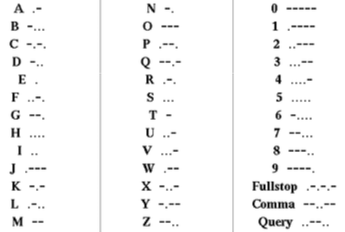
\includegraphics[scale=0.5]{apendice/problemas/problema1a/fig2.png}
\caption{Alfabeto \textit{Morse}}
\label{fig2}
\end{figure}

\subsection{Produto}
Um relatório no modelo de artigos da SBC com uma discussão detalhada sobre as três perguntas levantadas
e sobre a criptografia simplificada.
\subsection{Cronograma}

1 sessão tutorial e 1 aula expositiva.

\subsection{Recursos para aprendizagem}

\noindent
RAMOS, M. V. M.; JOSÉ NETO, J.; VEGA, I. S. \textbf{Linguagens Formais: Teoria, Modelagem e Implementação}. Editora Bookman, 2009.\\

\noindent
MENEZES, Paulo Blauth. \textbf{Linguagens formais e autômatos}. 6. ed. Bookman, 2011.\\

\subsection*{Referências}

Este problema é baseado no texto da Wilhelmiina Hamalainen\footnote{\url{https://www.researchgate.net/profile/Wilhelmiina_Haemaelaeinen}}.

\newpage
\section{\ProblemaH}
\subsection{Problema}
Os alunos da disciplina de Introdução as Linguagens Formais e Teoria da Computação normalmente
utilizam os computadores disponíveis em um dos laboratórios de informática da UFBA para
realização das atividades da disciplina.

Acontece que em um dia, os computadores de um destes laboratórios
de informática da UFBA começaram a apresentar um comportamento inesperado.

A primeira pessoa a relatar esse problema foi a Drissa.
Ela sentou de frente ao computador, como normalmente faz, mas ao digitar o próprio nome notou
que na tela estava escrito Qaxllo.
Ela tomou um susto sem entender o que estava acontecendo, então, como é amiga do Lucas, resolveu falar
com ele.
O Lucas estava sentado no computador ao lado, então ele tentou digitar Drissa no computador
que estava e percebeu que na tela apareceu Prsaaq.
O Lucas também tentou escrever o próprio nome e viu escrito na tela Dxwqa.

Então, Drissa e Lucas resolveram falar do problema para toda a turma, uma vez que não entenderam o
que estava acontecendo.
Em pouco tempo foi percebido que todos os computadores daquele laboratório estavam afetados
pelo problema.

A turma conversou rapidamente e percebeu que talvez este problema não seja muito difícil de resolver, então,
não precisariam esperar pelo atendimento do STI da UFBA, desta forma, resolveram fazer uma reunião para
discutir este problema e encontrar uma solução.

Quando todos já estavam saindo do laboratório para discutir o problema, o Angelmário, bastante atencioso,
alertou que não poderiam sair sem antes coletar mais informações para resolução do problema.
Então, assim foi feito, a Deuana e o Rodrigo foram os responsáveis por coletar o máximo de informações
possíveis.
Eles digitaram os nomes de todos os alunos da turma em cada um dos computadores e fizeram uma tabela de
correspondencia com o que era apresentado na tela.
Enquanto isso a Taiane disse que iria verificar se todos os cabos estavam
corretamente encaixados, ela constatou que todos os cabos estavam encaixados nos lugares certos.

\subsection{Produto}
Uma foto que demonstre que o problema está solucionado, bem como, um relatório que descreve os passos
para identificação e solução do problema, além de anexar todos os arquivos que julgar necessário.

\subsection{Cronograma}

1 sessão tutorial.

\subsection{Recursos para aprendizagem}
Não foram indicados recursos adicionais de aprendizagem.

\newpage
\section{\ProblemaI}
\subsection{Problema}
Os estudantes da disciplina de Introdução as Linguagens Formais e Teoria da Computação da UFBA
souberam na primeira aula da disciplina que será utilizada uma metodologia de ensino baseada
em problemas, então, eles resolveram pesquisar um pouco sobre a metodologia.

Os estudantes se reuniram para conversar sobre as coisas que tinham pesquisado.
Um dos estudantes disse que saber inferir informações implícitas em problemas é muito relevante
para que consigam obter bons resultados.
Outro estudante resolveu contar uma história e os demais ficaram atentos nos mínimos detalhes.

O estudante que conta a história diz que tudo começou na festa de aniversário da Alice.
Não, não a Alice do País das Maravilhas, mas uma amiga dele chamada de Alice:\\

--- Que tal preparar-nos umas tortas saborosas?---perguntou o Rei de Copas à Rainha de Copas num dia fresco de verão.

--- Fazer as tortas sem pimenta?---perguntou a Rainha.

--- Pimenta!---exclamou o Rei, incrédulo---Quer dizer que você usa pimenta em suas tortas?

--- Não muita---respondeu a Rainha.

--- E suponho que ela tem sido roubada!

--- É claro!---disse a Rainha---Encontre a pimenta e, quando descobrir quem a roubou, corte-lhe...

--- Vamos, vamos!---disse o Rei.

--- Bem, a pimenta tinha que ser encontrada, é claro. Agora, como todos vocês sabem, as pessoas que roubam pimenta nunca dizem a verdade.

--- O quê?!---disse Alice (não a Alice do País das Maravilhas, mas a Alice dessa festa)---Nunca ouvi falar disso antes!

--- Não ouviu?---perguntei-lhe, com falsa surpresa.

--- É claro que não! E tem mais, não acredito que ninguém mais tenha ouvido! Algum de vocês ouviu falar disso antes?

Todas as crianças abanaram a cabeça negativamente.

--- Bem,---disse eu---para fins desta história, vamos presumir que as pessoas que roubam pimenta nunca dizem a verdade.

--- Está bem---disse Alice, meio relutante.

--- Então, continuando a história, o suspeito mais óbvio era a cozinheira da Duquesa.

No julgamento, ela fez apenas uma declaração:

--- Eu sei quem roubou a pimenta!

--- Supondo que as pessoas que roubam a pi\-men\-ta sempre mentem, a cozinheira é culpada ou inocente?\\

PORTANTO, QUEM ROUBOU A PIMENTA?\\

Bem, os suspeitos seguintes do Rei foram a Lebre de Março, o Chapeleiro Louco e o Leirão. Os soldados foram mandados às casas deles, mas nenhuma pimenta foi encontrada. Mesmo assim, eles poderiam estar escondendo-a em algum lugar, de modo que foram detidos, com base nos princípios gerais.

No julgamento, a Lebre de Março afirmou que o Chapeleiro era inocente e o Chapeleiro afirmou que o Leirão era inocente. O Leirão resmungou uma declaração qualquer enquanto dormia, mas ela não foi registrada.

Como se constatou, nenhum inocente fizera uma afirmação falsa, e (como estamos lembrados) as pessoas que roubam pimenta nunca fazem afirmações verdadeiras. Além disso, a pimenta foi roubada por apenas uma criatura. Qual dos três é o culpado, se é que foi um deles?\\

ENTÃO, QUEM ROUBOU A PIMENTA?\\

--- Ora, ora, esse é realmente um caso difícil---disse o Rei.

Os suspeitos seguintes, curiosamente, foram o Grifo, a Falsa Tartaruga e a Lagosta.

No julgamento, o Grifo afirmou que a Falsa Tartaruga era inocente, e a Falsa Tartaruga disse que a Lagosta era culpada.
Mais uma vez, nenhum inocente mentiu e nenhum culpado disse a verdade.

Quem roubou a pimenta?

\subsection{Produto}
Um relatório no modelo de artigos da SBC para discutir se a cozinheira da história é culpada ou
inocente, se a Lebre de Março, o Chapeleiro Louco, o Leirão, o Grifo, a Falsa Tartaruga ou Lagosta
roubaram a pimenta.
É necessário detalhar cada inferência utilizada, por exemplo, ao inocentar ou acusar alguém, mostrar
quais as inferências e fatos utilizados para tal conclusão.

\subsection{Cronograma}
1 sessão tutorial.

\subsection{Recursos para aprendizagem}
Não foram indicados recursos adicionais de aprendizagem.

\section*{Referências}
Este problema é baseado no texto do Raymond Smullyan extraído do livro ``Alice no País dos Enigmas''.


% \include{apendice2}
% ...
% \include{apendiceM}

%% Fim do documento
\end{document}
%------------------------------------------------------------------------------------------%
